% Capitolul 0: Fundamente ale Analizei Seriilor de Timp
% Prezentare academică de calitate Harvard
% Program de licență, Academia de Studii Economice din București

\documentclass[9pt, aspectratio=169, t]{beamer}

% Asigură încadrarea conținutului pe diapozitive
\setbeamersize{text margin left=8mm, text margin right=8mm}

%=============================================================================
% CONFIGURARE TEMĂ ȘI STIL
%=============================================================================
\usetheme{default}
% Using default theme for clean header/footer control

% Color Palette (matching Redispatch PDF)
\definecolor{MainBlue}{RGB}{26, 58, 110}
\definecolor{AccentBlue}{RGB}{26, 58, 110}
\definecolor{IDAred}{RGB}{205, 0, 0}
\definecolor{DarkGray}{RGB}{51, 51, 51}
\definecolor{MediumGray}{RGB}{128, 128, 128}
\definecolor{LightGray}{RGB}{248, 248, 248}
\definecolor{VeryLightGray}{RGB}{235, 235, 235}
\definecolor{KeynoteGray}{RGB}{218, 218, 218}
\definecolor{SectionGray}{RGB}{120, 120, 120}
\definecolor{FooterGray}{RGB}{100, 100, 100}
\definecolor{Crimson}{RGB}{220, 53, 69}
\definecolor{Forest}{RGB}{46, 125, 50}
\definecolor{Amber}{RGB}{181, 133, 63}
\definecolor{Orange}{RGB}{230, 126, 34}
\definecolor{Purple}{RGB}{142, 68, 173}

% Gradient background (exact Keynote 315° gradient: white to RGB 218,218,218)
\setbeamertemplate{background}{%
    \begin{tikzpicture}[remember picture, overlay]
        \shade[shading=axis, shading angle=315,
        top color=white, bottom color=KeynoteGray]
        (current page.south west) rectangle (current page.north east);
    \end{tikzpicture}%
}
% Fallback solid color for compatibility
\setbeamercolor{background canvas}{bg=}

\setbeamercolor{palette primary}{bg=MainBlue, fg=white}
\setbeamercolor{palette secondary}{bg=MainBlue!85, fg=white}
\setbeamercolor{palette tertiary}{bg=MainBlue!70, fg=white}
\setbeamercolor{structure}{fg=MainBlue}
\setbeamercolor{title}{fg=IDAred}
\setbeamercolor{frametitle}{fg=IDAred, bg=}
\setbeamercolor{block title}{bg=MainBlue, fg=white}
\setbeamercolor{block body}{bg=VeryLightGray, fg=DarkGray}
\setbeamercolor{block title alerted}{bg=Crimson, fg=white}
\setbeamercolor{block body alerted}{bg=Crimson!8, fg=DarkGray}
\setbeamercolor{block title example}{bg=Forest, fg=white}
\setbeamercolor{block body example}{bg=Forest!8, fg=DarkGray}
\setbeamercolor{item}{fg=MainBlue}

% Footer colors (override Madrid theme blue)
\setbeamercolor{author in head/foot}{fg=FooterGray, bg=}
\setbeamercolor{title in head/foot}{fg=FooterGray, bg=}
\setbeamercolor{date in head/foot}{fg=FooterGray, bg=}
\setbeamercolor{section in head/foot}{fg=FooterGray, bg=}
\setbeamercolor{subsection in head/foot}{fg=FooterGray, bg=}

% Bullet styles (apply everywhere including blocks)
\setbeamertemplate{itemize item}{\color{MainBlue}$\boxdot$}
\setbeamertemplate{itemize subitem}{\color{MainBlue}$\blacktriangleright$}
\setbeamertemplate{itemize subsubitem}{\color{MainBlue}\tiny$\bullet$}
\setbeamertemplate{itemize/enumerate body begin}{\normalsize}
\setbeamertemplate{itemize/enumerate subbody begin}{\normalsize}

% Item spacing - compact style
\setlength{\leftmargini}{10pt}       % Level 1: minimal indent
\setlength{\leftmarginii}{10pt}      % Level 2: minimal additional indent
% Compact list spacing (zero extra space before/after lists in blocks)
\makeatletter
\def\@listi{\leftmargin\leftmargini \topsep 0pt \parsep 0pt \itemsep 0pt}
\def\@listii{\leftmargin\leftmarginii \topsep 0pt \parsep 0pt \itemsep 0pt}
\makeatother

\setbeamertemplate{navigation symbols}{}

%=============================================================================
% CUSTOM HEADLINE
%=============================================================================
\setbeamertemplate{headline}{%
    \vskip10pt%
    \hbox to \paperwidth{%
        \hskip0.5cm%
        {\small\color{FooterGray}\renewcommand{\hyperlink}[2]{##2}\insertsectionhead}%
        \hfill%
        \textcolor{FooterGray}{\small\insertframenumber}%
        \hskip0.5cm%
    }%
    \vskip4pt%
    {\color{FooterGray}\hrule height 0.4pt}%
}

%=============================================================================
% CUSTOM FOOTER
%=============================================================================
\usepackage{fontawesome5}

\setbeamertemplate{footline}{%
    {\color{FooterGray}\hrule height 0.4pt}%
    \vskip4pt%
    \hbox to \paperwidth{%
        \hskip0.5cm%
        \textcolor{FooterGray}{\small Analiza și Prognoza Seriilor de Timp}%
        \hfill%
        \raisebox{-0.1em}{%
            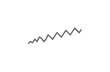
\begin{tikzpicture}[x=0.08em, y=0.08em, line width=0.4pt]
                \draw[FooterGray] (0,3) -- (1,4) -- (2,3.5) -- (3,5) -- (4,4) -- (5,6) -- (6,5.5) -- (7,4) -- (8,5) -- (9,7) -- (10,6) -- (11,5) -- (12,6.5) -- (13,8) -- (14,7) -- (15,6) -- (16,7.5) -- (17,9) -- (18,8) -- (19,7) -- (20,8.5) -- (21,10) -- (22,9) -- (23,8) -- (24,9.5);
            \end{tikzpicture}%
        }%
        \hskip0.5cm%
    }%
    \vskip6pt%
}

%=============================================================================
% PACHETE
%=============================================================================
\usepackage[utf8]{inputenc}
\usepackage[T1]{fontenc}
\usepackage{amsmath, amssymb, amsthm}
\usepackage{mathtools}
\usepackage{bm}
\usepackage{tikz}
\usetikzlibrary{arrows.meta, positioning, shapes, calc, decorations.pathreplacing, shadings}
\usepackage{booktabs}
\usepackage{multirow}
\usepackage{array}
\usepackage{graphicx}
\usepackage{hyperref}
\usepackage{colortbl}
\hypersetup{colorlinks=true, linkcolor=MainBlue, urlcolor=MainBlue}
\graphicspath{{../../logos/}{../../charts/}}
\hfuzz=2pt  % Suppress tiny overfull warnings (<2pt)
\vfuzz=2pt  % Suppress tiny vertical overfull warnings (<2pt)

%=============================================================================
% COMANDA QUANTLET
%=============================================================================
\newcommand{\quantlet}[2]{%
    \hfill\href{#2}{%
        \raisebox{-0.15em}{\includegraphics[height=0.7em]{ql_logo.png}}%
        \textcolor{MainBlue}{\tiny\ #1}%
    }%
}

%=============================================================================
% PAGINĂ TITLU PERSONALIZATĂ
%=============================================================================
\defbeamertemplate*{title page}{hybrid}[1][]
{
    \vspace{0.2cm}
    % Logos row - top header (with clickable links)
    \begin{center}
        \href{https://www.ase.ro}{\includegraphics[height=1.0cm]{ase_logo.png}}\hspace{0.3cm}%
        \href{https://theida.net}{\includegraphics[height=1.0cm]{ida_logo.png}}\hspace{0.3cm}%
        \href{https://blockchain-research-center.com}{\includegraphics[height=1.0cm]{brc_logo.png}}\hspace{0.3cm}%
        \href{https://www.ai4efin.ase.ro}{\includegraphics[height=1.0cm]{ai4efin_logo.png}}\hspace{0.3cm}%
        \href{https://ipe.ro/new}{\includegraphics[height=1.0cm]{acad_logo.png}}\hspace{0.3cm}%
        \href{https://www.digital-finance-msca.com}{\includegraphics[height=1.0cm]{msca_logo.png}}%
    \end{center}

    \vspace{0.6cm}

    % Main title with Q logos on sides (with clickable links)
    \begin{center}
        \begin{minipage}{0.1\textwidth}
            \centering
            \href{https://quantlet.com}{\includegraphics[height=1.1cm]{ql_logo.png}}
        \end{minipage}%
        \begin{minipage}{0.78\textwidth}
            \centering
            {\LARGE\bfseries\usebeamercolor[fg]{title}\inserttitle}

            \vspace{0.3cm}

            {\usebeamerfont{subtitle}\usebeamercolor[fg]{title}\insertsubtitle}
        \end{minipage}%
        \begin{minipage}{0.1\textwidth}
            \centering
            \href{https://quantinar.com}{\includegraphics[height=1.1cm]{qr_logo.png}}
        \end{minipage}
    \end{center}

    \vspace{0.6cm}

    % Authors (left aligned)
    \hspace{0.5cm}{\usebeamerfont{author}\insertauthor}

    \vspace{0.3cm}

    % Institute/Affiliations (left aligned)
    \hspace{0.5cm}\begin{minipage}[t]{0.9\textwidth}
        \raggedright\small\insertinstitute
    \end{minipage}
}

%=============================================================================
% MEDII PENTRU TEOREME
%=============================================================================
\theoremstyle{definition}
\setbeamertemplate{theorems}[numbered]
\newtheorem{defn}{Definiție}
\newtheorem{thm}{Teoremă}
\newtheorem{prop}{Propoziție}
\newtheorem{rmk}{Observație}

%=============================================================================
% COMENZI PERSONALIZATE
%=============================================================================
\newcommand{\E}{\mathbb{E}}
\newcommand{\Var}{\text{Var}}
\newcommand{\Cov}{\text{Cov}}
\newcommand{\Corr}{\text{Corr}}
\newcommand{\R}{\mathbb{R}}
\newcommand{\N}{\mathbb{N}}
\newcommand{\Z}{\mathbb{Z}}
\newcommand{\RMSE}{\text{RMSE}}
\newcommand{\MAE}{\text{MAE}}
\newcommand{\MAPE}{\text{MAPE}}

%=============================================================================
% INFORMAȚII TITLU
%=============================================================================
\title[Analiza Seriilor de Timp]{Analiza și Prognoza Seriilor de Timp}
\subtitle{Capitolul 0: Fundamente}
\author[D.T. Pele]{Daniel Traian PELE}
\institute{Academia de Studii Economice din București\\
IDA Institute Digital Assets\\
Blockchain Research Center\\
AI4EFin Artificial Intelligence for Energy Finance\\
Academia Română, Institutul de Prognoză Economică\\
MSCA Digital Finance}
\date{}

\begin{document}

% Title page (no header/footer)
{
\setbeamertemplate{headline}{}
\setbeamertemplate{footline}{}
\begin{frame}
    \titlepage
\end{frame}
}

%=============================================================================
% OBIECTIVE DE ÎNVĂȚARE
%=============================================================================
\begin{frame}{Obiective de învățare}
    \begin{block}{La sfârșitul acestui capitol, veți putea să:}
        \begin{itemize}\setlength{\itemsep}{2pt}
            \item[\textcolor{MainBlue}{\textbf{1.}}] \textbf{Definiți} seriile de timp și să le distingeți de datele transversale și de panel
            \item[\textcolor{MainBlue}{\textbf{2.}}] \textbf{Descompuneți} seriile de timp în componente de trend-ciclu, sezonalitate și reziduuri
            \item[\textcolor{MainBlue}{\textbf{3.}}] \textbf{Aplicați} metodele de netezire exponențială (SES, Holt, Holt-Winters, ETS)
            \item[\textcolor{MainBlue}{\textbf{4.}}] \textbf{Evaluați} prognozele folosind MAE, RMSE, MAPE, sMAPE
            \item[\textcolor{MainBlue}{\textbf{5.}}] \textbf{Implementați} separarea train/validare/test și validarea încrucișată
            \item[\textcolor{MainBlue}{\textbf{6.}}] \textbf{Modelați} sezonalitatea folosind variabile dummy sau termeni Fourier
            \item[\textcolor{MainBlue}{\textbf{7.}}] \textbf{Eliminați} trendul și sezonalitatea prin metode adecvate
            \item[\textcolor{MainBlue}{\textbf{8.}}] \textbf{Distingeți} între trendurile deterministe și stochastice
        \end{itemize}
    \end{block}
\end{frame}

%=============================================================================
% SURSE DE DATE ȘI INSTRUMENTE SOFTWARE
%=============================================================================
\begin{frame}{Surse de date și instrumente software}
    \begin{columns}[T]
        \begin{column}{0.48\textwidth}
            \begin{block}{Surse de date}
                \begin{itemize}\setlength{\itemsep}{0pt}
                    \item \textbf{Yahoo Finance}
                    \begin{itemize}
                        \item Prețuri acțiuni, criptomonede, valute
                    \end{itemize}
                    \item \textbf{FRED} (Federal Reserve)
                    \begin{itemize}
                        \item PIB, șomaj, rate dobânzi
                    \end{itemize}
                    \item \textbf{Eurostat / INS / BNR}
                    \begin{itemize}
                        \item Date economice europene și românești
                    \end{itemize}
                    \item \textbf{Seturi clasice}
                    \begin{itemize}
                        \item AirPassengers, Sunspots, CO$_2$
                    \end{itemize}
                \end{itemize}
            \end{block}
        \end{column}
        \begin{column}{0.48\textwidth}
            \begin{exampleblock}{Python}
                \begin{itemize}\setlength{\itemsep}{0pt}
                    \item \texttt{yfinance} — date Yahoo Finance
                    \item \texttt{pandas\_datareader} — FRED, Eurostat
                    \item \texttt{statsmodels} — modele statistice
                    \item \texttt{pandas} — manipulare date
                    \item \texttt{matplotlib} — vizualizare
                \end{itemize}
            \end{exampleblock}
            \vspace{0.1cm}
            \begin{alertblock}{R}
                \begin{itemize}\setlength{\itemsep}{0pt}
                    \item \texttt{quantmod} — date financiare
                    \item \texttt{tseries} — teste serii de timp
                    \item \texttt{forecast} — modele de prognoză
                    \item \texttt{fredr} — acces FRED API
                \end{itemize}
            \end{alertblock}
        \end{column}
    \end{columns}
\end{frame}

%=============================================================================
% CUPRINS
%=============================================================================
\begin{frame}{Structura capitolului}
    \setbeamertemplate{section in toc}{\color{MainBlue}$\boxdot$~\inserttocsection}
    \tableofcontents
\end{frame}

%=============================================================================
% MOTIVAȚIE
%=============================================================================
\section{Motivație}

\begin{frame}{Seriile de timp sunt pretutindeni}
    \vspace{-0.3cm}
    \begin{center}
        \includegraphics[width=0.95\textwidth, height=0.60\textheight, keepaspectratio]{ch1_motivation_everywhere.png}
    \end{center}
    \vspace{-2mm}
    \quantlet{TSA\_ch0\_real\_data}{https://github.com/QuantLet/TSA/tree/main/TSA_ch0/TSA_ch0_real_data}
    \vspace{-0.2cm}
    {\footnotesize
    \begin{itemize}
        \item \textbf{Finanțe}: Prețuri acțiuni, cursuri valutare, volume
        \item \textbf{Economie}: PIB, șomaj, rate ale inflației
        \item \textbf{Business}: Vânzări, trafic website, cerere
        \item \textbf{Știință}: Temperatură, poluare, semne vitale
    \end{itemize}
    }
\end{frame}

\begin{frame}{De ce studiem seriile de timp?}
    \vspace{-0.2cm}
    \begin{center}
        \includegraphics[width=0.95\textwidth, height=0.52\textheight, keepaspectratio]{ch1_motivation_forecast.png}
    \end{center}
    \vspace{-2mm}
    \quantlet{TSA\_ch0\_real\_data}{https://github.com/QuantLet/TSA/tree/main/TSA_ch0/TSA_ch0_real_data}
    \vspace{-0.3cm}
    {\footnotesize
    \begin{alertblock}{Obiectiv principal: prognoza}
        \begin{itemize}\setlength{\itemsep}{0pt}
            \item Folosim tiparele istorice pentru a prezice valori viitoare $\succ$ esențial pentru planificarea afacerilor, managementul riscului și deciziile de politică
        \end{itemize}
    \end{alertblock}
    }
\end{frame}

\begin{frame}{Înțelegerea structurii seriilor de timp}
    \vspace{-0.2cm}
    \begin{center}
        \includegraphics[width=0.92\textwidth, height=0.52\textheight, keepaspectratio]{ch1_motivation_components.png}
    \end{center}
    \vspace{-2mm}
    \quantlet{TSA\_ch0\_real\_data}{https://github.com/QuantLet/TSA/tree/main/TSA_ch0/TSA_ch0_real_data}
    \vspace{-0.3cm}
    {\footnotesize
    \begin{exampleblock}{Descompunere}
        \begin{itemize}\setlength{\itemsep}{0pt}
            \item Orice serie de timp poate fi descompusă în: \textbf{trend-ciclu} + \textbf{sezonalitate} + \textbf{zgomot}
        \end{itemize}
    \end{exampleblock}
    }
\end{frame}

%=============================================================================
% SECȚIUNEA 1: CE ESTE O SERIE DE TIMP
%=============================================================================
\section{Ce Este o Serie de timp?}

\begin{frame}{Definiția unei serii de timp}
    \begin{defn}[Serie de timp]
        \begin{itemize}\setlength{\itemsep}{0pt}
            \item \textbf{Serie de timp}: secvență de observații $\{X_t\}$ indexate după timp:
            $\{X_t : t \in \mathcal{T}\}$
            unde $\mathcal{T}$ este o mulțime de indici reprezentând momente de timp
        \end{itemize}
    \end{defn}

    \vspace{0.2cm}

    \begin{columns}[T]
        \column{0.5\textwidth}
        \begin{block}{Caracteristici cheie}
            \begin{itemize}\setlength{\itemsep}{0pt}
                \item \textbf{Ordonate}: ordine temporală naturală
                \item \textbf{Dependente}: observațiile consecutive sunt corelate
                \item \textbf{Discrete/Continue}: $t = 1, 2, 3, \ldots$
            \end{itemize}
        \end{block}

        \column{0.5\textwidth}
        \begin{exampleblock}{Notație}
            \begin{itemize}\setlength{\itemsep}{0pt}
                \item \textbf{$X_t$}: observația la momentul $t$
                \item \textbf{$\{X_t\}_{t=1}^{T}$}: serie cu $T$ observații
            \end{itemize}
        \end{exampleblock}
    \end{columns}
\end{frame}

\begin{frame}{Serie de timp: ilustrație conceptuală}
    \begin{columns}[T]
        \column{0.35\textwidth}
        \begin{exampleblock}{Elemente fundamentale}
            \begin{itemize}\setlength{\itemsep}{0pt}
                \item \textbf{Notație formală}
                \begin{itemize}
                    \item $X_t$ = valoarea la momentul $t$
                    \item $t \in \{1, 2, \ldots, T\}$
                \end{itemize}
                \item \textbf{Autocorelație}
                \begin{itemize}
                    \item $\rho_k = \text{Corr}(X_t, X_{t-k})$
                    \item Măsoară dependența temporală
                \end{itemize}
            \end{itemize}
        \end{exampleblock}
        \column{0.63\textwidth}
        \vspace{-0.3cm}
        \begin{center}
            \includegraphics[width=\textwidth, height=0.78\textheight, keepaspectratio]{ch1_def_timeseries.pdf}
        \end{center}
        \vspace{-2mm}
        \quantlet{TSA\_ch0\_definition}{https://github.com/QuantLet/TSA/tree/main/TSA_ch0/TSA_ch0_definition}
    \end{columns}
\end{frame}

\begin{frame}{Tipare comune în seriile de timp}
    \begin{columns}[T]
        \column{0.38\textwidth}
        \begin{block}{Tipuri de tipare}
            \begin{itemize}\setlength{\itemsep}{0pt}
                \item \textbf{Trend}
                \begin{itemize}
                    \item Creștere sau scădere pe termen lung
                \end{itemize}
                \item \textbf{Sezonier}
                \begin{itemize}
                    \item Tipare periodice regulate
                \end{itemize}
                \item \textbf{Ciclic}
                \begin{itemize}
                    \item Fluctuații pe termen mediu (2--10 ani)
                \end{itemize}
                \item \textbf{Aleatoriu}
                \begin{itemize}
                    \item Fluctuații imprevizibile
                \end{itemize}
            \end{itemize}
        \end{block}
        \column{0.60\textwidth}
        \vspace{-0.3cm}
        \begin{center}
            \includegraphics[width=\textwidth, height=0.75\textheight, keepaspectratio]{ch1_ts_patterns.pdf}
        \end{center}
        \vspace{-2mm}
        \quantlet{TSA\_ch0\_definition}{https://github.com/QuantLet/TSA/tree/main/TSA_ch0/TSA_ch0_definition}
    \end{columns}
\end{frame}

\begin{frame}{Exemplu practic: date financiare reale}
    \begin{columns}[T]
        \column{0.35\textwidth}
        \begin{block}{S\&P 500 (2024)}
            \begin{itemize}\setlength{\itemsep}{0pt}
                \item \textbf{Frecvență zilnică}
                \begin{itemize}
                    \item $\approx$ 252 zile de tranzacționare/an
                \end{itemize}
                \item \textbf{Caracteristici observate}
                \begin{itemize}
                    \item Trend ascendent
                    \item Volatilitate în clustere
                    \item Persistență (momentum)
                \end{itemize}
            \end{itemize}
        \end{block}
        \column{0.63\textwidth}
        \vspace{-0.3cm}
        \begin{center}
            \includegraphics[width=\textwidth, height=0.78\textheight, keepaspectratio]{timeseries_definition.pdf}
        \end{center}
        \vspace{-2mm}
        \quantlet{TSA\_ch0\_definition}{https://github.com/QuantLet/TSA/tree/main/TSA_ch0/TSA_ch0_definition}
    \end{columns}
\end{frame}

\begin{frame}{Tipuri de date: comparație}
    \begin{center}
        \includegraphics[width=0.95\textwidth, height=0.52\textheight, keepaspectratio]{data_types_comparison.png}
    \end{center}
    \vspace{-0.2cm}
    \begin{center}
    \small
    \begin{tabular}{lccc}
        \toprule
        \textbf{Tip de Date} & \textbf{Unități ($N$)} & \textbf{Timp ($T$)} & \textbf{Exemplu} \\
        \midrule
        Transversale & Multe & 1 & Sondaj pe 1000 gospodării \\
        Serie de timp & 1 & Multe & Prețuri zilnice S\&P 500 \\
        Panel & Multe & Multe & PIB-ul a 50 țări, 20 ani \\
        \bottomrule
    \end{tabular}
    \end{center}
    \vspace{-2mm}
    \quantlet{TSA\_ch0\_definition}{https://github.com/QuantLet/TSA/tree/main/TSA_ch0/TSA_ch0_definition}
\end{frame}

\begin{frame}{Exemple de date de tip serie de timp}
    \begin{columns}[T]
        \column{0.35\textwidth}
        \begin{exampleblock}{Date financiare reale}
            \begin{itemize}\setlength{\itemsep}{0pt}
                \item \textbf{Sursă}: Yahoo Finance (2019--2025)
                \begin{itemize}
                    \item Normalizate la baza 100
                \end{itemize}
                \item \textbf{Bitcoin}: cel mai volatil
                \item \textbf{Aur}: cel mai stabil
            \end{itemize}
        \end{exampleblock}
        \column{0.63\textwidth}
        \vspace{-0.3cm}
        \begin{center}
            \includegraphics[width=\textwidth, height=0.78\textheight, keepaspectratio]{multiple_assets.pdf}
        \end{center}
        \vspace{-2mm}
        \quantlet{TSA\_ch0\_real\_data}{https://github.com/QuantLet/TSA/tree/main/TSA_ch0/TSA_ch0_real_data}
    \end{columns}
\end{frame}

%=============================================================================
% SECȚIUNEA 2: DESCOMPUNEREA SERIILOR DE TIMP
%=============================================================================
\section{Descompunerea seriilor de timp}

\begin{frame}{De ce descompunem o serie de timp?}
    \vspace{-0.2cm}
    \begin{columns}[T]
        \begin{column}{0.48\textwidth}
            \begin{block}{Obiective}
                \begin{itemize}\setlength{\itemsep}{0pt}
                    \item Înțelegerea tiparelor subiacente
                    \item Eliminarea sezonalității pentru modelare
                    \item Identificarea direcției trendului
                    \item Izolarea fluctuațiilor neregulate
                    \item Îmbunătățirea acurateții prognozei
                \end{itemize}
            \end{block}
        \end{column}
        \begin{column}{0.48\textwidth}
            \begin{exampleblock}{Componente}
                \begin{itemize}\setlength{\itemsep}{0pt}
                    \item \textbf{$T_t$}: Trend-Ciclu
                    \begin{itemize}
                        \item Mișcare pe termen lung
                    \end{itemize}
                    \item \textbf{$S_t$}: Sezonier
                    \begin{itemize}
                        \item Tipar periodic regulat
                    \end{itemize}
                    \item \textbf{$\varepsilon_t$}: Reziduu
                    \begin{itemize}
                        \item Zgomot aleatoriu
                    \end{itemize}
                \end{itemize}
            \end{exampleblock}
        \end{column}
    \end{columns}

    \vspace{0.1cm}

    \begin{block}{Modele clasice de descompunere}
        \begin{itemize}\setlength{\itemsep}{0pt}
            \item \textbf{Aditiv}: $X_t = T_t + S_t + \varepsilon_t$
            \begin{itemize}
                \item Amplitudine sezonieră constantă
            \end{itemize}
            \item \textbf{Multiplicativ}: $X_t = T_t \times S_t \times \varepsilon_t$
            \begin{itemize}
                \item Amplitudine sezonieră crește cu nivelul
            \end{itemize}
        \end{itemize}
    \end{block}
\end{frame}

\begin{frame}{Descompunerea seriilor de timp: exemplu vizual}
    \begin{columns}[T]
        \column{0.35\textwidth}
        \begin{block}{Componente explicate}
            \begin{itemize}\setlength{\itemsep}{0pt}
                \item \textbf{Original}
                \begin{itemize}
                    \item Seria observată
                \end{itemize}
                \item \textbf{Trend-Ciclu}
                \begin{itemize}
                    \item Mișcare pe termen lung
                \end{itemize}
                \item \textbf{Sezonier}
                \begin{itemize}
                    \item Tipar periodic
                \end{itemize}
                \item \textbf{Reziduu}
                \begin{itemize}
                    \item Zgomot aleatoriu
                \end{itemize}
            \end{itemize}
        \end{block}
        \column{0.63\textwidth}
        \vspace{-0.3cm}
        \begin{center}
            \includegraphics[width=\textwidth, height=0.78\textheight, keepaspectratio]{ch1_decomposition.png}
        \end{center}
        \vspace{-2mm}
        \quantlet{TSA\_ch0\_decomposition}{https://github.com/QuantLet/TSA/tree/main/TSA_ch0/TSA_ch0_decomposition}
    \end{columns}
\end{frame}

\begin{frame}{Componenta ciclică}
    \vspace{-0.3cm}
    \begin{center}
        \includegraphics[width=0.95\textwidth, height=0.50\textheight, keepaspectratio]{ch1_cyclical_component.png}
    \end{center}
        \vspace{-2mm}
        \quantlet{TSA\_ch0\_decomposition}{https://github.com/QuantLet/TSA/tree/main/TSA_ch0/TSA_ch0_decomposition}
    \vspace{-0.2cm}
    {\small
    \begin{columns}[T]
        \column{0.48\textwidth}
        \begin{block}{Caracteristici}
            \begin{itemize}\setlength{\itemsep}{0pt}
                \item \textbf{Durată}: fluctuații pe termen mediu (2--10 ani)
                \item \textbf{Aperiodic}: fără perioadă fixă (vs sezonalitate)
                \item \textbf{Origine}: reflectă ciclurile economice
            \end{itemize}
        \end{block}

        \column{0.48\textwidth}
        \begin{alertblock}{În practică}
            \begin{itemize}\setlength{\itemsep}{0pt}
                \item \textbf{Combinare}: ciclul combinat cu trendul
                \item \textbf{Dificultate}: greu de identificat în serii scurte
                \item \textbf{Soluție}: de obicei absorbit în trend-ciclu
            \end{itemize}
        \end{alertblock}
    \end{columns}
    }
\end{frame}

\begin{frame}{Modelul de descompunere aditivă}
    \begin{block}{Model}
        \begin{itemize}\setlength{\itemsep}{0pt}
            \item \textbf{Ecuație}: $X_t = T_t + S_t + \varepsilon_t$
            \begin{itemize}
                \item Componentele se adună pentru a forma seria observată
            \end{itemize}
        \end{itemize}
    \end{block}

    \vspace{0.2cm}

    \begin{columns}[T]
        \column{0.48\textwidth}
        \begin{exampleblock}{Când să folosim}
            \begin{itemize}\setlength{\itemsep}{0pt}
                \item \textbf{Fluctuații sezoniere constante}
                \begin{itemize}
                    \item Amplitudinea nu depinde de nivel
                \end{itemize}
                \item \textbf{Varianța seriei stabilă}
                \begin{itemize}
                    \item Măsoară dispersia în jurul mediei
                    \item Estimator: $s^2 = \frac{1}{n-1}\sum_{i=1}^n (x_i - \bar{x})^2$
                \end{itemize}
            \end{itemize}
        \end{exampleblock}

        \column{0.48\textwidth}
        \begin{block}{Proprietăți}
            \begin{itemize}\setlength{\itemsep}{0pt}
                \item \textbf{Eroare}: $\E[\varepsilon_t] = 0$ (medie zero)
                \item \textbf{Sezonier}: $\sum_{j=1}^{s} S_j = 0$ (suma sezonală e zero)
                \item \textbf{Unități}: $S_t$ sunt aceleași ca $X_t$
            \end{itemize}
        \end{block}
    \end{columns}
\end{frame}

\begin{frame}{Descompunere aditivă: vizualizare}
    \vspace{-0.3cm}
    \begin{center}
        \includegraphics[width=0.95\textwidth, height=0.52\textheight, keepaspectratio]{ts_components_synthetic.png}
    \end{center}
    \vspace{-3mm}
    \quantlet{TSA\_ch0\_decomposition}{https://github.com/QuantLet/TSA/tree/main/TSA_ch0/TSA_ch0_decomposition}
    \vspace{-2mm}
    \begin{block}{Interpretare}
        \begin{itemize}\setlength{\itemsep}{0pt}
            \item \textbf{Descompunere}: Original = Trend + Sezonier + Reziduu
            \item \textbf{Proprietate}: amplitudine sezonieră constantă, nu depinde de nivel
        \end{itemize}
    \end{block}
\end{frame}

\begin{frame}{Modelul de descompunere multiplicativă}
    \vspace{-0.3cm}
    \begin{block}{Model}
        \begin{itemize}\setlength{\itemsep}{0pt}
            \item \textbf{Ecuație}: $X_t = T_t \times S_t \times \varepsilon_t$ $\succ$ componentele se înmulțesc
        \end{itemize}
    \end{block}

    \vspace{0.05cm}

    {\footnotesize
    \begin{columns}[T]
        \column{0.48\textwidth}
        \begin{exampleblock}{Când să folosim}
            \begin{itemize}\setlength{\itemsep}{0pt}
                \item \textbf{Fluctuații crescătoare}: sezonalitatea crește cu nivelul
                \item \textbf{Heteroscedasticitate}: varianța crește în timp
                \item \textbf{Exemple}: date economice/financiare
            \end{itemize}
        \end{exampleblock}

        \column{0.48\textwidth}
        \begin{block}{Proprietăți}
            \begin{itemize}\setlength{\itemsep}{0pt}
                \item \textbf{Eroare}: $\E[\varepsilon_t] = 1$ (centrat la 1)
                \item \textbf{Sezonier}: $\frac{1}{s}\sum_{j=1}^{s} S_j = 1$ (media e 1)
                \item \textbf{Unități}: $S_t$ este raport adimensional
            \end{itemize}
        \end{block}
    \end{columns}
    }

    \vspace{0.05cm}

    {\footnotesize
    \begin{alertblock}{Sfat}
        \begin{itemize}\setlength{\itemsep}{0pt}
            \item \textbf{Transformare logaritmică}: multiplicativ $\succ$ aditiv: $\log X_t = \log T_t + \log S_t + \log \varepsilon_t$
        \end{itemize}
    \end{alertblock}
    }
\end{frame}

\begin{frame}{Descompunere multiplicativă: date reale}
    \begin{center}
        \includegraphics[width=0.85\textwidth, height=0.48\textheight, keepaspectratio]{airline_decomposition.pdf}
    \end{center}
    \vspace{-3mm}
    {\footnotesize
    \begin{exampleblock}{Exemplu}
        \begin{itemize}\setlength{\itemsep}{0pt}
            \item Date Box-Jenkins: pasageri lunari (1949--1960). Amplitudinea sezonieră crește cu nivelul
        \end{itemize}
    \end{exampleblock}
    }
    \quantlet{TSA\_ch0\_decomposition}{https://github.com/QuantLet/TSA/tree/main/TSA_ch0/TSA_ch0_decomposition}
\end{frame}

\begin{frame}{Aditivă vs multiplicativă: comparație}
    \begin{columns}[T]
        \column{0.35\textwidth}
        \begin{block}{Diferența cheie}
            \begin{itemize}\setlength{\itemsep}{0pt}
                \item \textbf{Multiplicativ}
                \begin{itemize}
                    \item Componenta sezonieră este un \textit{raport}
                    \item Centrată la valoarea 1
                \end{itemize}
                \item \textbf{Aditiv}
                \begin{itemize}
                    \item Componenta sezonieră în \textit{unități absolute}
                    \item Centrată la valoarea 0
                \end{itemize}
            \end{itemize}
        \end{block}
        \column{0.63\textwidth}
        \vspace{-0.3cm}
        \begin{center}
            \includegraphics[width=\textwidth, height=0.78\textheight, keepaspectratio]{additive_vs_multiplicative.pdf}
        \end{center}
        \vspace{-2mm}
        \quantlet{TSA\_ch0\_decomposition}{https://github.com/QuantLet/TSA/tree/main/TSA_ch0/TSA_ch0_decomposition}
    \end{columns}
\end{frame}

\begin{frame}{Estimarea trendului: media mobilă}
    \begin{defn}[media mobilă centrată]
        \begin{itemize}\setlength{\itemsep}{0pt}
            \item \textbf{Media mobilă centrată} de ordin $2q+1$:
            \vspace{-0.2cm}
            \begin{equation}
                \hat{T}_t = \frac{1}{2q+1} \sum_{j=-q}^{q} X_{t+j}
            \end{equation}
            \vspace{-0.3cm}
        \end{itemize}
    \end{defn}

    \vspace{0.2cm}

    \begin{columns}[T]
        \column{0.48\textwidth}
        \begin{block}{Pentru date sezoniere}
            \begin{itemize}\setlength{\itemsep}{0pt}
                \item \textbf{Perioada $s$ impară}
                \begin{itemize}
                    \item Se folosește medie simplă
                \end{itemize}
                \item \textbf{Perioada $s$ pară}
                \begin{itemize}
                    \item $2 \times s$ MA cu ponderi jumătate
                \end{itemize}
            \end{itemize}
        \end{block}

        \column{0.48\textwidth}
        \begin{exampleblock}{Proprietăți}
            \begin{itemize}\setlength{\itemsep}{0pt}
                \item \textbf{Netezire}: elimină sezonierul \& aleatoriul
                \item \textbf{Fereastră mare} $\succ$ estimare mai netedă
                \item \textbf{Dezavantaj}: pierdere de date la extremități
            \end{itemize}
        \end{exampleblock}
    \end{columns}
\end{frame}

\begin{frame}{Media mobilă centrată: ilustrație vizuală}
    \begin{center}
        \includegraphics[width=0.85\textwidth, height=0.52\textheight, keepaspectratio]{ch1_def_moving_average.pdf}
    \end{center}
    \vspace{-2mm}
    \begin{exampleblock}{Interpretare}
        \begin{itemize}\setlength{\itemsep}{0pt}
            \item \textbf{Netezire}: elimină fluctuațiile pe termen scurt
            \item \textbf{Rezultat}: dezvăluie trendul subiacent
        \end{itemize}
    \end{exampleblock}
    \quantlet{TSA\_ch0\_definition}{https://github.com/QuantLet/TSA/tree/main/TSA_ch0/TSA_ch0_definition}
\end{frame}

\begin{frame}{Algoritmul descompunerii clasice}
    \begin{block}{Pași pentru descompunerea multiplicativă}
        \begin{itemize}\setlength{\itemsep}{0pt}
            \item \textbf{Pasul 1} $\succ$ \textbf{Estimare Trend}: $\hat{T}_t = MA_s(X_t)$
            \begin{itemize}
                \item Medie mobilă centrată de ordinul perioadei sezoniere
            \end{itemize}
            \item \textbf{Pasul 2} $\succ$ \textbf{Eliminarea trendului}: $D_t = X_t / \hat{T}_t$
            \item \textbf{Pasul 3} $\succ$ \textbf{Estimare Sezonier}: $\hat{S}_j = \text{media}(D_t \text{ pentru sezonul } j)$
            \item \textbf{Pasul 4} $\succ$ \textbf{Normalizare}: scalare astfel încât $\frac{1}{s}\sum_{j=1}^{s} \hat{S}_j = 1$
            \item \textbf{Pasul 5} $\succ$ \textbf{Calcul Reziduuri}: $\hat{\varepsilon}_t = X_t / (\hat{T}_t \times \hat{S}_t)$
        \end{itemize}
    \end{block}

    \vspace{0.3cm}

    \begin{alertblock}{Notă}
        \begin{itemize}\setlength{\itemsep}{0pt}
            \item \textbf{Pentru descompunere aditivă}: operațiile se modifică
            \begin{itemize}
                \item Împărțire $\succ$ scădere
                \item Înmulțire $\succ$ adunare
            \end{itemize}
        \end{itemize}
    \end{alertblock}
\end{frame}

\begin{frame}{Indici sezonieri: interpretare}
    \begin{center}
        \includegraphics[width=0.85\textwidth, height=0.48\textheight, keepaspectratio]{seasonal_pattern.pdf}
    \end{center}
    \vspace{-3mm}
    {\footnotesize
    \begin{exampleblock}{Interpretare}
        \begin{itemize}\setlength{\itemsep}{0pt}
            \item $S_t > 1$: activitate peste medie; $S_t < 1$: sub medie. Vârf de călătorii în iulie--august
        \end{itemize}
    \end{exampleblock}
    }
    \quantlet{TSA\_ch0\_seasonal}{https://github.com/QuantLet/TSA/tree/main/TSA_ch0/TSA_ch0_seasonal}
\end{frame}

\begin{frame}{Descompunerea STL: o abordare modernă}
    \begin{defn}[STL - Descompunere Sezonier-Trend folosind LOESS]
        \begin{itemize}\setlength{\itemsep}{0pt}
            \item \textbf{STL}: folosește regresie locală ponderată (LOESS): $X_t = T_t + S_t + R_t$
        \end{itemize}
    \end{defn}

    \vspace{0.1cm}

    \begin{columns}[T]
        \column{0.5\textwidth}
        \begin{exampleblock}{Avantaje}
            \begin{itemize}\setlength{\itemsep}{0pt}
                \item \textbf{Flexibilitate}: orice perioadă sezonieră
                \item \textbf{Variabilitate}: sezonalitatea poate evolua în timp
                \item \textbf{Robustețe}: rezistentă la valori extreme
                \item \textbf{Netezire}: estimări netede ale trendului
            \end{itemize}
        \end{exampleblock}

        \column{0.5\textwidth}
        \begin{block}{Parametri cheie}
            \begin{itemize}\setlength{\itemsep}{0pt}
                \item \textbf{\texttt{period}}: perioada sezonieră
                \begin{itemize}
                    \item Ex: 12 pentru date lunare, 4 pentru trimestriale
                \end{itemize}
                \item \textbf{\texttt{seasonal}}: fereastra de netezire
                \item \textbf{\texttt{robust}}: ponderare redusă pentru outlieri
            \end{itemize}
        \end{block}
    \end{columns}
\end{frame}

\begin{frame}{Descompunerea STL: ilustrație vizuală}
    \begin{center}
        \includegraphics[width=0.85\textwidth, height=0.48\textheight, keepaspectratio]{ch1_def_stl.pdf}
    \end{center}
    \vspace{-3mm}
    {\footnotesize
    \begin{block}{Idee cheie}
        \begin{itemize}\setlength{\itemsep}{0pt}
            \item STL (Seasonal-Trend-Loess): separă trend + sezonier + rest folosind regresie LOESS
        \end{itemize}
    \end{block}
    }
    \quantlet{TSA\_ch0\_decomposition}{https://github.com/QuantLet/TSA/tree/main/TSA_ch0/TSA_ch0_decomposition}
\end{frame}

%=============================================================================
% SECȚIUNEA 3: METODE DE NETEZIRE EXPONENȚIALĂ
%=============================================================================
\section{Metode de Netezire Exponențială}

\begin{frame}{Netezirea exponențială: prezentare generală}
    \begin{block}{Definiție}
        \begin{itemize}\setlength{\itemsep}{0pt}
            \item \textbf{Netezirea exponențială}: medii ponderate ale observațiilor trecute
            \begin{itemize}
                \item Ponderile scad exponențial în timp
                \item Observațiile recente primesc ponderi mai mari
            \end{itemize}
        \end{itemize}
    \end{block}

    \vspace{0.2cm}

    \begin{columns}[T]
        \column{0.5\textwidth}
        \begin{exampleblock}{De ce netezire exponențială?}
            \begin{itemize}\setlength{\itemsep}{0pt}
                \item \textbf{Simplă}: ușor de implementat și înțeles
                \begin{itemize}
                    \item Un singur parametru de netezire
                \end{itemize}
                \item \textbf{Adaptivă}: ponderi mai mari pentru date recente
                \item \textbf{Versatilă}: gestionează trend și sezonalitate
            \end{itemize}
        \end{exampleblock}

        \column{0.5\textwidth}
        \begin{alertblock}{Trei metode principale}
            \begin{itemize}\setlength{\itemsep}{0pt}
                \item \textbf{SES} (Simple Exponential Smoothing): doar nivel
                \begin{itemize}
                    \item Cea mai simplă metodă exponențială
                \end{itemize}
                \item \textbf{Holt}: nivel + trend
                \begin{itemize}
                    \item Captează direcția de evoluție
                \end{itemize}
                \item \textbf{Holt-Winters}: + sezonalitate
                \begin{itemize}
                    \item Model complet cu toate componentele
                \end{itemize}
            \end{itemize}
        \end{alertblock}
    \end{columns}
\end{frame}

\begin{frame}{Netezirea cu media mobilă}
    \vspace{-0.3cm}
    \begin{center}
        \includegraphics[width=0.85\textwidth, height=0.48\textheight, keepaspectratio]{ch1_moving_average.png}
    \end{center}
    \vspace{-3mm}
    \begin{block}{Compromisul dimensiunii ferestrei}
        \begin{itemize}\setlength{\itemsep}{0pt}
            \item \textbf{Fereastră mică}: reactivă dar zgomotoasă
            \begin{itemize}
                \item Captează schimbări rapide, dar amplifică zgomotul
            \end{itemize}
            \item \textbf{Fereastră mare}: netedă dar cu întârziere
            \begin{itemize}
                \item Elimină zgomotul, dar reacționează lent
            \end{itemize}
        \end{itemize}
    \end{block}
    \quantlet{TSA\_ch0\_definition}{https://github.com/QuantLet/TSA/tree/main/TSA_ch0/TSA_ch0_definition}
\end{frame}

\begin{frame}{Netezirea exponențială simplă (SES)}
    \begin{block}{Model}
        \begin{itemize}\setlength{\itemsep}{0pt}
            \item \textbf{Ecuație}: $\hat{X}_{t+1|t} = \alpha X_t + (1-\alpha)\hat{X}_{t|t-1}$
            \begin{itemize}
                \item $\alpha \in (0,1)$ este parametrul de netezire
            \end{itemize}
        \end{itemize}
    \end{block}

    \vspace{0.2cm}

    \begin{columns}[T]
        \column{0.5\textwidth}
        \begin{exampleblock}{Cum funcționează}
            \begin{itemize}\setlength{\itemsep}{0pt}
                \item \textbf{Principiu}: ponderile scad exponențial
                \item \textbf{$\alpha$ mare}
                \begin{itemize}
                    \item Prognoză reactivă la schimbări
                \end{itemize}
                \item \textbf{$\alpha$ mic}
                \begin{itemize}
                    \item Prognoză mai netedă, stabilă
                \end{itemize}
            \end{itemize}
        \end{exampleblock}

        \column{0.5\textwidth}
        \begin{block}{Forma cu nivel}
            \begin{itemize}\setlength{\itemsep}{0pt}
                \item \textbf{Ecuație}: $\ell_t = \alpha X_t + (1-\alpha)\ell_{t-1}$
                \begin{itemize}
                    \item $\ell_t$ = nivelul estimat la momentul $t$
                    \item Prognoză: $\hat{X}_{t+h|t} = \ell_t$ (constantă)
                \end{itemize}
            \end{itemize}
        \end{block}
    \end{columns}
\end{frame}

\begin{frame}{Netezirea exponențială simplă: efectul lui $\alpha$}
    \vspace{-0.3cm}
    \begin{center}
        \includegraphics[width=0.85\textwidth, height=0.48\textheight, keepaspectratio]{simple_exp_smoothing.pdf}
    \end{center}
    \vspace{-3mm}
    \begin{exampleblock}{Compromis}
        \begin{itemize}\setlength{\itemsep}{0pt}
            \item \textbf{$\alpha$ mic} $\succ$ prognoze netede
            \begin{itemize}
                \item Mai multă pondere pe istoria îndepărtată
            \end{itemize}
            \item \textbf{$\alpha$ mare} $\succ$ urmărește datele
            \begin{itemize}
                \item Reacție rapidă la schimbări recente
            \end{itemize}
        \end{itemize}
    \end{exampleblock}
    \quantlet{TSA\_ch0\_smoothing}{https://github.com/QuantLet/TSA/tree/main/TSA_ch0/TSA_ch0_smoothing}
\end{frame}

\begin{frame}{SES: exemplu numeric pas cu pas}
    \vspace{-0.3cm}
    {\footnotesize
    \begin{exampleblock}{Date: Vânzări lunare (mii EUR)}
        \vspace{-0.1cm}
        \begin{itemize}\setlength{\itemsep}{0pt}
            \item \textbf{Date}: $X_1=100,\; X_2=110,\; X_3=105,\; X_4=115,\; X_5=120$ \quad ($\alpha=0.3$, $\hat{X}_{1|0}=100$)
        \end{itemize}
        \vspace{-0.1cm}
    \end{exampleblock}
    \vspace{-0.2cm}
    \begin{block}{Calcul iterativ: $\hat{X}_{t+1|t} = \alpha X_t + (1-\alpha)\hat{X}_{t|t-1}$}
        \vspace{-0.1cm}
        \renewcommand{\arraystretch}{1.1}
        \begin{tabular}{ccccl}
            \toprule
            $t$ & $X_t$ & $\hat{X}_{t|t-1}$ & $e_t$ & Calcul $\hat{X}_{t+1|t}$ \\
            \midrule
            1 & 100 & 100.00 & 0.00 & $0.3 \times 100 + 0.7 \times 100 = \mathbf{100.00}$ \\
            2 & 110 & 100.00 & 10.00 & $0.3 \times 110 + 0.7 \times 100 = \mathbf{103.00}$ \\
            3 & 105 & 103.00 & 2.00 & $0.3 \times 105 + 0.7 \times 103 = \mathbf{103.60}$ \\
            4 & 115 & 103.60 & 11.40 & $0.3 \times 115 + 0.7 \times 103.6 = \mathbf{107.02}$ \\
            5 & 120 & 107.02 & 12.98 & $0.3 \times 120 + 0.7 \times 107.02 = \mathbf{110.91}$ \\
            \bottomrule
        \end{tabular}
        \vspace{-0.1cm}
    \end{block}
    \vspace{-0.2cm}
    \begin{alertblock}{Prognoză și evaluare}
        \vspace{-0.1cm}
        $\hat{X}_{6|5} = \mathbf{110.91}$ \quad
        MAE $= 7.28$ \quad
        RMSE $= 8.97$
        \vspace{-0.1cm}
    \end{alertblock}
    }
\end{frame}

\begin{frame}{Metoda Holt cu trend liniar}
    \begin{block}{Ecuații}
        \begin{itemize}\setlength{\itemsep}{0pt}
            \item \textbf{Nivel}: $\ell_t = \alpha X_t + (1-\alpha)(\ell_{t-1} + b_{t-1})$
            \item \textbf{Trend}: $b_t = \beta^*(\ell_t - \ell_{t-1}) + (1-\beta^*)b_{t-1}$
            \item \textbf{Prognoză}: $\hat{X}_{t+h|t} = \ell_t + h \cdot b_t$
            \begin{itemize}
                \item Extrapolează trendul liniar pe $h$ pași
            \end{itemize}
        \end{itemize}
    \end{block}

    \vspace{0.1cm}

    \begin{columns}[T]
        \column{0.5\textwidth}
        \begin{exampleblock}{Parametri}
            \begin{itemize}\setlength{\itemsep}{0pt}
                \item \textbf{$\alpha$}: netezire nivel
                \begin{itemize}
                    \item Controlează reactivitatea la schimbări de nivel
                \end{itemize}
                \item \textbf{$\beta^*$}: netezire trend
                \begin{itemize}
                    \item Controlează reactivitatea la schimbări de pantă
                \end{itemize}
            \end{itemize}
        \end{exampleblock}

        \column{0.5\textwidth}
        \begin{block}{Componente}
            \begin{itemize}\setlength{\itemsep}{0pt}
                \item \textbf{$\ell_t$}: nivel estimat
                \begin{itemize}
                    \item Media locală a seriei
                \end{itemize}
                \item \textbf{$b_t$}: trend estimat (pantă)
                \begin{itemize}
                    \item Rata de creștere/descreștere
                \end{itemize}
            \end{itemize}
        \end{block}
    \end{columns}
\end{frame}

\begin{frame}{Metoda Holt: vizualizare}
    \begin{columns}[T]
        \column{0.35\textwidth}
        \begin{exampleblock}{Interpretare}
            \begin{itemize}\setlength{\itemsep}{0pt}
                \item \textbf{Metoda Holt}: captează nivelul și trendul
                \begin{itemize}
                    \item Le proiectează în orizontul de prognoză
                \end{itemize}
                \item \textbf{$\alpha$}: controlează schimbări de nivel
                \item \textbf{$\beta^*$}: controlează schimbări de trend
            \end{itemize}
        \end{exampleblock}
        \vspace{0.2cm}
        
        \column{0.63\textwidth}
        \vspace{-0.3cm}
        \begin{center}
            \includegraphics[width=\textwidth, height=0.78\textheight, keepaspectratio]{holt_method.pdf}
        \end{center}
        \vspace{-2mm}
        \quantlet{TSA\_ch0\_smoothing}{https://github.com/QuantLet/TSA/tree/main/TSA_ch0/TSA_ch0_smoothing}
    \end{columns}
\end{frame}

\begin{frame}{Metoda sezonieră Holt-Winters}
    \begin{block}{Ecuații (Sezonalitate aditivă)}
        \begin{itemize}\setlength{\itemsep}{0pt}
            \item \textbf{Nivel}: $\ell_t = \alpha(X_t - S_{t-s}) + (1-\alpha)(\ell_{t-1} + b_{t-1})$
            \item \textbf{Trend}: $b_t = \beta^*(\ell_t - \ell_{t-1}) + (1-\beta^*)b_{t-1}$
            \item \textbf{Sezonier}: $S_t = \gamma(X_t - \ell_t) + (1-\gamma)S_{t-s}$
            \item \textbf{Prognoză}: $\hat{X}_{t+h|t} = \ell_t + h \cdot b_t + S_{t+h-s(k+1)}$
            \begin{itemize}
                \item Unde $k = \lfloor(h-1)/s\rfloor$
            \end{itemize}
        \end{itemize}
    \end{block}

    \vspace{0.1cm}

    \begin{exampleblock}{Parametri}
        \begin{itemize}\setlength{\itemsep}{0pt}
            \item \textbf{$\alpha$} — nivel
            \item \textbf{$\beta^*$} — trend
            \item \textbf{$\gamma$} — sezonier
            \item \textbf{$s$} — perioadă sezonieră
            \begin{itemize}
                \item Toți în $(0, 1)$; estimați prin minimizarea erorii
            \end{itemize}
        \end{itemize}
    \end{exampleblock}
\end{frame}

\begin{frame}{Holt-Winters: captarea sezonalității}
    \begin{columns}[T]
        \column{0.32\textwidth}
        \begin{exampleblock}{Caracteristică cheie}
            \begin{itemize}\setlength{\itemsep}{0pt}
                \item \textbf{Descompunere completă}
                \begin{itemize}
                    \item Separă nivel, trend și sezonier
                \end{itemize}
                \item \textbf{Prognoze sezoniere}
                \begin{itemize}
                    \item Include atât trend cât și tipar periodic
                \end{itemize}
            \end{itemize}
        \end{exampleblock}
        \column{0.66\textwidth}
        \vspace{-0.3cm}
        \begin{center}
            \includegraphics[width=\textwidth, height=0.80\textheight, keepaspectratio]{holt_winters.pdf}
        \end{center}
        \vspace{-2mm}
        \quantlet{TSA\_ch0\_smoothing}{https://github.com/QuantLet/TSA/tree/main/TSA_ch0/TSA_ch0_smoothing}
    \end{columns}
\end{frame}

\begin{frame}{Cadrul ETS: eroare-trend-sezonalitate}
    \vspace{-0.3cm}
    \begin{defn}[Modele ETS]
        \begin{itemize}\setlength{\itemsep}{0pt}
            \item \textbf{Cadrul ETS}: generalizează netezirea exponențială: ETS$(E, T, S)$
        \end{itemize}
    \end{defn}

    \vspace{-0.1cm}

    {\footnotesize
    \begin{center}
    \begin{tabular}{llll}
        \toprule
        \textbf{Componentă} & \textbf{N} & \textbf{A} & \textbf{M} \\
        \midrule
        Eroare (E) & -- & aditivă & multiplicativă \\
        Trend (T) & Niciunul & Aditiv & Multiplicativ \\
        Sezonier (S) & Niciunul & Aditiv & Multiplicativ \\
        \bottomrule
    \end{tabular}
    \end{center}
    }

    \vspace{0.05cm}

    {\footnotesize
    \begin{exampleblock}{Exemple}
        \begin{itemize}\setlength{\itemsep}{0pt}
            \item \textbf{ETS(A,N,N)}: Netezire exponențială simplă $\succ$ doar nivel, fără trend sau sezonalitate
            \item \textbf{ETS(A,A,N)}: Metoda Liniară Holt $\succ$ nivel + trend aditiv
            \item \textbf{ETS(A,A,A)}: Holt-Winters aditivă $\succ$ nivel + trend + sezonalitate aditivă
        \end{itemize}
    \end{exampleblock}
    }
\end{frame}

\begin{frame}{ETS: ilustrație netezire exponențială}
    \begin{center}
        \includegraphics[width=0.85\textwidth, height=0.48\textheight, keepaspectratio]{ch1_def_ets.pdf}
    \end{center}
    \vspace{-3mm}
    {\footnotesize
    \begin{exampleblock}{Interpretare}
        \begin{itemize}\setlength{\itemsep}{0pt}
            \item Observații ponderate exponențial: ponderile scad cu vechimea; observațiile recente au importanță mai mare
        \end{itemize}
    \end{exampleblock}
    }
    \quantlet{TSA\_ch0\_smoothing}{https://github.com/QuantLet/TSA/tree/main/TSA_ch0/TSA_ch0_smoothing}
\end{frame}

\begin{frame}{Selecția modelului ETS}
    \begin{columns}[T]
        \column{0.32\textwidth}
        \begin{exampleblock}{Selecție automată}
            \begin{itemize}\setlength{\itemsep}{0pt}
                \item \textbf{Criterii informaționale}
                \begin{itemize}
                    \item AIC (Akaike Information Criterion)
                    \item BIC (Bayesian Information Criterion)
                \end{itemize}
                \item \textbf{Selecție optimală}
                \begin{itemize}
                    \item Balanță între ajustare și complexitate
                \end{itemize}
            \end{itemize}
        \end{exampleblock}
        \column{0.66\textwidth}
        \vspace{-0.3cm}
        \begin{center}
            \includegraphics[width=\textwidth, height=0.80\textheight, keepaspectratio]{ets_components.pdf}
        \end{center}
        \vspace{-2mm}
        \quantlet{TSA\_ch0\_smoothing}{https://github.com/QuantLet/TSA/tree/main/TSA_ch0/TSA_ch0_smoothing}
    \end{columns}
\end{frame}

\begin{frame}{Metode cu trend amortizat}
    \begin{block}{Parametrul de amortizare}
        \begin{itemize}\setlength{\itemsep}{0pt}
            \item \textbf{Parametru}: $\phi \in (0,1)$
            \begin{itemize}
                \item Previne supra-proiecția trendului
                \item Trendul converge către o constantă
            \end{itemize}
        \end{itemize}
    \end{block}

    \vspace{0.1cm}

    \begin{columns}[T]
        \column{0.55\textwidth}
        \begin{block}{Ecuații}
            \begin{itemize}\setlength{\itemsep}{0pt}
                \item \textbf{Nivel}: $\ell_t = \alpha X_t + (1-\alpha)(\ell_{t-1} + \phi b_{t-1})$
                \item \textbf{Trend}: $b_t = \beta^*(\ell_t - \ell_{t-1}) + (1-\beta^*)\phi b_{t-1}$
                \item \textbf{Prognoză}: $\hat{X}_{t+h|t} = \ell_t + \phi\frac{1-\phi^h}{1-\phi}b_t$
            \end{itemize}
        \end{block}
        \column{0.43\textwidth}
        \begin{exampleblock}{Idee cheie}
            \begin{itemize}\setlength{\itemsep}{0pt}
                \item \textbf{Asimptotic}: când $h \to \infty$, prognoza $\to$ constantă
                \begin{itemize}
                    \item Previne extrapolare nerealistă pe termen lung
                \end{itemize}
                \item \textbf{Avantaj}: adesea mai bună pentru orizonturi lungi
            \end{itemize}
        \end{exampleblock}
    \end{columns}
\end{frame}

%=============================================================================
% SECȚIUNEA 4: EVALUAREA PROGNOZEI
%=============================================================================
\section{Evaluarea prognozei}

\begin{frame}{Metrici de acuratețe a prognozei}
    \vspace{-0.3cm}
    {\footnotesize
    \begin{block}{Eroarea de prognoză}
        \begin{itemize}\setlength{\itemsep}{0pt}
            \item \textbf{Definiție}: $e_t = X_t - \hat{X}_t$ (actual minus prezis)
            \begin{itemize}
                \item Pozitivă $\Rightarrow$ subestimează; Negativă $\Rightarrow$ supraestimează
            \end{itemize}
        \end{itemize}
    \end{block}
    }

    \vspace{0.05cm}

    {\footnotesize
    \begin{columns}[T]
        \begin{column}{0.48\textwidth}
            \begin{block}{Dependente de scală}
                \begin{itemize}\setlength{\itemsep}{0pt}
                    \item \textbf{MAE}: $\frac{1}{n}\sum|e_t|$
                    \item \textbf{MSE}: $\frac{1}{n}\sum e_t^2$
                    \item \textbf{RMSE}: $\sqrt{\text{MSE}}$
                \end{itemize}
            \end{block}
        \end{column}
        \begin{column}{0.48\textwidth}
            \begin{block}{Independente de scală}
                \begin{itemize}\setlength{\itemsep}{0pt}
                    \item \textbf{MAPE}: $\frac{100}{n}\sum\left|\frac{e_t}{X_t}\right|$
                    \item \textbf{sMAPE}: $\frac{100}{n}\sum\frac{|e_t|}{(|X_t|+|\hat{X}_t|)/2}$
                \end{itemize}
            \end{block}
        \end{column}
    \end{columns}
    }

    \vspace{0.05cm}

    {\footnotesize
    \begin{alertblock}{Ce să folosim?}
        \begin{itemize}\setlength{\itemsep}{0pt}
            \item \textbf{Aceeași serie}: RMSE, MAE $\succ$ comparare modele pe aceleași date
            \item \textbf{Între serii diferite}: MAPE, sMAPE $\succ$ metrici procentuale, independente de scală
        \end{itemize}
    \end{alertblock}
    }
\end{frame}

\begin{frame}{Evaluarea prognozei: exemplu vizual}
    \begin{columns}[T]
        \column{0.35\textwidth}
        \begin{block}{Observații}
            \begin{itemize}\setlength{\itemsep}{2pt}
                \item \textbf{Sus}: actual vs.\ prognoză
                \begin{itemize}
                    \item Evaluare vizuală a calității prognozei
                \end{itemize}
                \item \textbf{Jos}: reziduuri
                \begin{itemize}
                    \item Medie zero
                    \item Varianță constantă
                    \item Fără tipar
                \end{itemize}
            \end{itemize}
        \end{block}
        \column{0.63\textwidth}
        \begin{center}
            \includegraphics[width=\textwidth, height=0.78\textheight, keepaspectratio]{ch1_forecast_eval.png}
        \end{center}
    \end{columns}
    \vspace{-2mm}
    \quantlet{TSA\_ch0\_forecast\_eval}{https://github.com/QuantLet/TSA/tree/main/TSA_ch0/TSA_ch0_forecast_eval}
\end{frame}

\begin{frame}{Compararea metodelor de prognoză}
    \begin{center}
        \includegraphics[width=0.85\textwidth, height=0.48\textheight, keepaspectratio]{forecast_accuracy_metrics.pdf}
    \end{center}
    \vspace{-3mm}
    {\footnotesize
    \begin{exampleblock}{Interpretare}
        \begin{itemize}\setlength{\itemsep}{0pt}
            \item \textbf{Stânga}: Prognoze SES, Holt, Holt-Winters. \textbf{Dreapta}: Metrici de eroare. Comparație vizuală și cantitativă
        \end{itemize}
    \end{exampleblock}
    }
    \quantlet{TSA\_ch0\_forecast\_eval}{https://github.com/QuantLet/TSA/tree/main/TSA_ch0/TSA_ch0_forecast_eval}
\end{frame}

\begin{frame}{Diagnosticarea reziduurilor}
    \begin{columns}[T]
        \column{0.48\textwidth}
        \begin{block}{Proprietăți ale reziduurilor}
            \begin{itemize}\setlength{\itemsep}{0pt}
                \item \textbf{Medie zero}: $\E[e_t] = 0$
                \begin{itemize}
                    \item Prognoza nu are bias sistematic
                \end{itemize}
                \item \textbf{Necorelate}: $\Cov(e_t, e_{t-k}) = 0$
                \begin{itemize}
                    \item Nu rămâne informație neexploatată
                \end{itemize}
                \item \textbf{Varianță constantă}: $\Var(e_t) = \sigma^2$
                \item \textbf{Normal distribuite}: pentru intervale de încredere
            \end{itemize}
        \end{block}
        \column{0.5\textwidth}
        \begin{exampleblock}{Teste de diagnostic}
            \begin{itemize}\setlength{\itemsep}{0pt}
                \item \textbf{Testul Ljung-Box} (autocorelație):
                \begin{itemize}
                    \item $Q = T(T+2)\sum_{k=1}^{h}\frac{\hat{\rho}_k^2}{T-k} \sim \chi^2_h$
                \end{itemize}
                \item \textbf{Testul Jarque-Bera} (normalitate):
                \begin{itemize}
                    \item $JB = \frac{T}{6}\left(S^2 + \frac{(K-3)^2}{4}\right) \sim \chi^2_2$
                    \item $S$ = asimetrie, $K$ = curtosis
                \end{itemize}
            \end{itemize}
        \end{exampleblock}
    \end{columns}
\end{frame}

\begin{frame}{Diagnosticarea reziduurilor: vizualizare}
    \begin{columns}[T]
        \column{0.32\textwidth}
        \begin{exampleblock}{Ce să verificăm}
            \begin{itemize}\setlength{\itemsep}{0pt}
                \item \textbf{Grafic temporal}: fără tipare sistematice
                \item \textbf{Histogramă}: verificare normalitate
                \item \textbf{ACF}: fără autocorelație semnificativă
                \item \textbf{Grafic Q-Q}: confirmare normalitate
            \end{itemize}
        \end{exampleblock}
        \column{0.66\textwidth}
        \vspace{-0.3cm}
        \begin{center}
            \includegraphics[width=\textwidth, height=0.75\textheight, keepaspectratio]{residual_diagnostics.pdf}
        \end{center}
        \vspace{-2mm}
        \quantlet{TSA\_ch0\_forecast\_eval}{https://github.com/QuantLet/TSA/tree/main/TSA_ch0/TSA_ch0_forecast_eval}
    \end{columns}
\end{frame}

\begin{frame}{Validarea încrucișată pentru serii de timp}
    \begin{columns}[T]
        \begin{column}{0.48\textwidth}
            \begin{alertblock}{De ce nu CV standard?}
                \begin{itemize}\setlength{\itemsep}{0pt}
                    \item \textbf{Dependență temporală}: observațiile sunt corelate
                    \item \textbf{Ordinea contează}: trebuie respectată cronologia
                    \item \textbf{K-fold standard} $\succ$ data leakage
                \end{itemize}
            \end{alertblock}
        \end{column}
        \begin{column}{0.48\textwidth}
            \begin{block}{CV (cross-validation) cu origine mobilă}
                \begin{itemize}\setlength{\itemsep}{0pt}
                    \item \textbf{Pasul 1}: antrenare pe $\{X_1, \ldots, X_t\}$
                    \item \textbf{Pasul 2}: prognoză $\hat{X}_{t+h}$
                    \item \textbf{Pasul 3}: incrementare $t$, repetare
                \end{itemize}
            \end{block}
        \end{column}
    \end{columns}

    \begin{center}
        \includegraphics[width=0.95\textwidth, height=0.42\textheight, keepaspectratio]{cross_validation_forecast.png}
    \end{center}
        \vspace{-2mm}
        \quantlet{TSA\_ch0\_forecast\_eval}{https://github.com/QuantLet/TSA/tree/main/TSA_ch0/TSA_ch0_forecast_eval}
\end{frame}

\begin{frame}{Separarea train / validare / test}
    \vspace{-0.2cm}
    \begin{columns}[T]
        \begin{column}{0.32\textwidth}
            \begin{block}{Set de Antrenare}
                \begin{itemize}\setlength{\itemsep}{0pt}
                    \item Potrivirea parametrilor modelului
                    \item Cea mai mare porțiune (60--80\%)
                    \item Folosit pentru estimare
                \end{itemize}
            \end{block}
        \end{column}
        \begin{column}{0.32\textwidth}
            \begin{exampleblock}{Set de Validare}
                \begin{itemize}\setlength{\itemsep}{0pt}
                    \item Ajustarea hiperparametrilor
                    \item Compararea modelelor
                    \item Selectarea celei mai bune abordări
                \end{itemize}
            \end{exampleblock}
        \end{column}
        \begin{column}{0.32\textwidth}
            \begin{alertblock}{Set de Test}
                \begin{itemize}\setlength{\itemsep}{0pt}
                    \item Doar evaluare finală
                    \item Niciodată folosit pentru ajustare
                    \item Performanță imparțială
                \end{itemize}
            \end{alertblock}
        \end{column}
    \end{columns}

    \vspace{0.1cm}

    \begin{center}
        \includegraphics[width=0.55\textwidth]{train_test_validation.png}
    \end{center}
        \vspace{-2mm}
        \quantlet{TSA\_ch0\_forecast\_eval}{https://github.com/QuantLet/TSA/tree/main/TSA_ch0/TSA_ch0_forecast_eval}
\end{frame}

\begin{frame}{Fluxul de lucru pentru dezvoltarea modelului}
    \begin{center}
    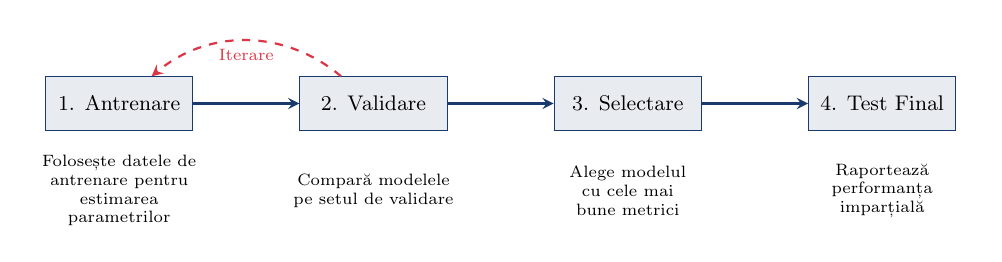
\begin{tikzpicture}[node distance=1.8cm, scale=0.85, transform shape]
        \tikzstyle{process} = [rectangle, minimum width=2.2cm, minimum height=0.8cm, text centered, draw=MainBlue, fill=MainBlue!10, font=\small]
        \tikzstyle{arrow} = [->, >=stealth, thick, MainBlue]

        % Nodes
        \node (train) [process] {1. Antrenare};
        \node (validate) [process, right of=train, xshift=2cm] {2. Validare};
        \node (select) [process, right of=validate, xshift=2cm] {3. Selectare};
        \node (test) [process, right of=select, xshift=2cm] {4. Test Final};

        % Arrows
        \draw [arrow] (train) -- (validate);
        \draw [arrow] (validate) -- (select);
        \draw [arrow] (select) -- (test);

        % Feedback loop
        \draw [arrow, dashed, Crimson] (validate) to[bend right=40] node[below, font=\scriptsize] {Iterare} (train);

        % Labels below
        \node [below of=train, yshift=0.5cm, font=\scriptsize, text width=2.5cm, align=center] {Folosește datele de\\antrenare pentru\\estimarea parametrilor};
        \node [below of=validate, yshift=0.5cm, font=\scriptsize, text width=2.5cm, align=center] {Compară modelele\\pe setul de validare};
        \node [below of=select, yshift=0.5cm, font=\scriptsize, text width=2.5cm, align=center] {Alege modelul\\cu cele mai bune metrici};
        \node [below of=test, yshift=0.5cm, font=\scriptsize, text width=2.5cm, align=center] {Raportează\\performanța imparțială};
    \end{tikzpicture}
    \end{center}

    \vspace{0.15cm}

    \begin{alertblock}{Regulă critică}
        \begin{itemize}\setlength{\itemsep}{0pt}
            \item \textbf{Niciodată testul pentru selecție!}
            \begin{itemize}
                \item Folosiți doar pentru evaluare finală
            \end{itemize}
            \item \textbf{Evitați scurgerea de date}
            \begin{itemize}
                \item Estimări prea optimiste ale performanței
            \end{itemize}
        \end{itemize}
    \end{alertblock}
\end{frame}

\begin{frame}{Date reale: compararea prognozelor}
    \begin{columns}[T]
        \column{0.32\textwidth}
        \begin{exampleblock}{Interpretare}
            \begin{itemize}\setlength{\itemsep}{0pt}
                \item \textbf{Date}: pasageri companii aeriene
                \item \textbf{Cel mai bun}: Holt-Winters multiplicativă
                \begin{itemize}
                    \item Ideal pentru date cu sezonalitate crescătoare
                \end{itemize}
            \end{itemize}
        \end{exampleblock}
        \column{0.66\textwidth}
        \vspace{-0.3cm}
        \begin{center}
            \includegraphics[width=\textwidth, height=0.80\textheight, keepaspectratio]{real_data_forecast_comparison.pdf}
        \end{center}
        \vspace{-2mm}
        \quantlet{TSA\_ch0\_forecast\_eval}{https://github.com/QuantLet/TSA/tree/main/TSA_ch0/TSA_ch0_forecast_eval}
    \end{columns}
\end{frame}

\begin{frame}{Performanța prognozei pe diferite seturi de date}
    \begin{columns}[T]
        \column{0.32\textwidth}
        \begin{exampleblock}{Interpretare}
            \begin{itemize}\setlength{\itemsep}{0pt}
                \item \textbf{Serii diferite}
                \begin{itemize}
                    \item Necesită modele diferite
                \end{itemize}
                \item \textbf{Date sezoniere}
                \begin{itemize}
                    \item Preferați metode sezoniere
                \end{itemize}
                \item \textbf{Nu există model universal}
                \begin{itemize}
                    \item Testați mai multe abordări
                \end{itemize}
            \end{itemize}
        \end{exampleblock}
        \column{0.66\textwidth}
        \vspace{-0.3cm}
        \begin{center}
            \includegraphics[width=\textwidth, height=0.80\textheight, keepaspectratio]{multiple_series_comparison.pdf}
        \end{center}
        \vspace{-2mm}
        \quantlet{TSA\_ch0\_forecast\_eval}{https://github.com/QuantLet/TSA/tree/main/TSA_ch0/TSA_ch0_forecast_eval}
    \end{columns}
\end{frame}

%=============================================================================
% SECȚIUNEA 5: MODELAREA SEZONALITĂȚII
%=============================================================================
\section{Modelarea sezonalității}

\begin{frame}{Modelarea sezonalității: două abordări}
    \vspace{-0.2cm}
    \begin{columns}[T]
        \begin{column}{0.48\textwidth}
            \begin{block}{1. Variabile dummy}
                \begin{itemize}\setlength{\itemsep}{0pt}
                    \item \textbf{Model}: $X_t = \mu + \sum_{j=1}^{s-1}\gamma_j D_{jt} + \varepsilon_t$
                    \item $D_{jt} = 1$ dacă $t$ în sezonul $j$
                    \item $s-1$ parametri
                    \item Orice tipar sezonier
                \end{itemize}
            \end{block}
        \end{column}
        \begin{column}{0.48\textwidth}
            \begin{exampleblock}{2. Termeni Fourier}
                \begin{itemize}\setlength{\itemsep}{0pt}
                    \item {\small \textbf{Model}: $X_t = \mu + \sum_{k=1}^{K}\!\left[\alpha_k\sin\!\left(\frac{2\pi k t}{s}\right) + \beta_k\cos\!\left(\frac{2\pi k t}{s}\right)\right]$}
                    \item Funcții sinusoidale
                    \item $2K$ parametri
                    \item Tipare netede
                \end{itemize}
            \end{exampleblock}
        \end{column}
    \end{columns}

    \vspace{0.1cm}

    \begin{alertblock}{Compromis}
        \begin{itemize}\setlength{\itemsep}{0pt}
            \item \textbf{Variabile dummy}
            \begin{itemize}
                \item Orice tipar sezonier, dar mai mulți parametri
            \end{itemize}
            \item \textbf{Termeni Fourier}
            \begin{itemize}
                \item Tipare netede, mai puțini parametri
            \end{itemize}
        \end{itemize}
    \end{alertblock}
\end{frame}

\begin{frame}{Variabile dummy vs termeni Fourier}
    \begin{columns}[T]
        \column{0.35\textwidth}
        \begin{block}{Comparație}
            \begin{itemize}\setlength{\itemsep}{0pt}
                \item \textbf{Variabile dummy}
                \begin{itemize}
                    \item Captează orice formă
                    \item Necesită $s-1$ parametri
                \end{itemize}
                \item \textbf{Termeni Fourier}
                \begin{itemize}
                    \item Doar $2K$ parametri
                    \item Tipare netede, sinusoidale
                \end{itemize}
            \end{itemize}
        \end{block}
        \column{0.63\textwidth}
        \vspace{-0.3cm}
        \begin{center}
            \includegraphics[width=\textwidth, height=0.78\textheight, keepaspectratio]{seasonality_fourier_dummies.pdf}
        \end{center}
        \vspace{-2mm}
        \quantlet{TSA\_ch0\_seasonal}{https://github.com/QuantLet/TSA/tree/main/TSA_ch0/TSA_ch0_seasonal}
    \end{columns}
\end{frame}

\begin{frame}{Alegerea între dummy și Fourier}
    \begin{center}
    \small
    \begin{tabular}{lcc}
        \toprule
        \textbf{Criteriu} & \textbf{Dummy} & \textbf{Fourier} \\
        \midrule
        Parametri (lunar) & 11 & $2K$ (adesea 4--6) \\
        Tipar sezonier & Orice formă & Neted/sinusoidal \\
        Interpretare & Directă (efecte lunare) & Componente de frecvență \\
        Sezoane de înaltă frecvență & Mulți parametri & Eficient \\
        Sezonalitate multiplă & Complex & Ușor (adăugați termeni) \\
        \bottomrule
    \end{tabular}
    \end{center}

    \vspace{0.1cm}

    \begin{exampleblock}{Recomandări}
        \begin{itemize}\setlength{\itemsep}{0pt}
            \item \textbf{Folosiți Dummy}
            \begin{itemize}
                \item Tipare neregulate, coeficienți interpretabili
            \end{itemize}
            \item \textbf{Folosiți Fourier}
            \begin{itemize}
                \item Tipare netede, sezonalitate de înaltă frecvență
                \item Utilizat în TBATS și Prophet
            \end{itemize}
        \end{itemize}
    \end{exampleblock}
\end{frame}

%=============================================================================
% SECȚIUNEA 6: GESTIONAREA TRENDULUI ȘI SEZONALITĂȚII
%=============================================================================
\section{Gestionarea Trendului și Sezonalității}

\begin{frame}{De ce eliminăm trendul și sezonalitatea?}
    \vspace{-0.2cm}
    \begin{columns}[T]
        \begin{column}{0.48\textwidth}
            \begin{block}{Motive pentru eliminarea trendului}
                \begin{itemize}\setlength{\itemsep}{0pt}
                    \item Cerința de staționaritate
                    \item Focus pe fluctuații
                    \item Evitarea regresiei false
                    \item Permiterea inferenței valide
                \end{itemize}
            \end{block}
        \end{column}
        \begin{column}{0.48\textwidth}
            \begin{exampleblock}{Motive pentru desezonalizare}
                \begin{itemize}\setlength{\itemsep}{0pt}
                    \item Dezvăluirea trendului subiacent
                    \item Comparații între sezoane
                    \item Simplificarea modelării
                    \item Focus pe componenta neregulată
                \end{itemize}
            \end{exampleblock}
        \end{column}
    \end{columns}

    \vspace{0.1cm}

    \begin{alertblock}{Important}
        \begin{itemize}\setlength{\itemsep}{0pt}
            \item \textbf{Modelăm seria transformată}
            \begin{itemize}
                \item Cu trendul și sezonalitatea eliminate
            \end{itemize}
            \item \textbf{Inversăm transformarea}
            \begin{itemize}
                \item Readucem prognoza la scala originală
            \end{itemize}
        \end{itemize}
    \end{alertblock}
\end{frame}

\begin{frame}{Metode de eliminare a trendului}
    \begin{columns}[T]
        \column{0.55\textwidth}
        \begin{block}{Șase abordări comune de eliminare a trendului}
            \begin{itemize}\setlength{\itemsep}{0pt}
                \item \textbf{Diferențiere}: $\Delta X_t = X_t - X_{t-1}$
                \begin{itemize}
                    \item Cea mai utilizată, elimină trend stochastic
                \end{itemize}
                \item \textbf{Regresie liniară}: $\hat{T}_t = \hat{\beta}_0 + \hat{\beta}_1 t$
                \item \textbf{Polinomială}: polinom de ordin superior
                \item \textbf{Filtru HP}: echilibru estimare vs netezime
                \item \textbf{Media mobilă}: $\hat{T}_t = MA_q(X_t)$
                \item \textbf{LOESS}: regresie polinomială locală
            \end{itemize}
        \end{block}
        \column{0.43\textwidth}
        \begin{exampleblock}{Alegerea depinde de}
            \begin{itemize}\setlength{\itemsep}{0pt}
                \item \textbf{Natura trendului}
                \begin{itemize}
                    \item Determinist vs stochastic
                \end{itemize}
                \item \textbf{Scopul analizei}
                \begin{itemize}
                    \item Prognoză vs analiză descriptivă
                \end{itemize}
            \end{itemize}
        \end{exampleblock}
    \end{columns}
\end{frame}

\begin{frame}{Metode de eliminarea trendului: comparație}
    \begin{columns}[T]
        \column{0.32\textwidth}
        \begin{alertblock}{Idee cheie}
            \begin{itemize}\setlength{\itemsep}{0pt}
                \item \textbf{Metode diferite}
                \begin{itemize}
                    \item Produc reziduuri diferite
                \end{itemize}
                \item \textbf{Alegere după tipul de trend}
                \begin{itemize}
                    \item Considerați obiectivele analizei
                \end{itemize}
            \end{itemize}
        \end{alertblock}
        \column{0.66\textwidth}
        \vspace{-0.3cm}
        \begin{center}
            \includegraphics[width=\textwidth, height=0.80\textheight, keepaspectratio]{detrending_methods.pdf}
        \end{center}
        \vspace{-2mm}
        \quantlet{TSA\_ch0\_detrending}{https://github.com/QuantLet/TSA/tree/main/TSA_ch0/TSA_ch0_detrending}
    \end{columns}
\end{frame}

\begin{frame}{Estimarea trendului: abordări multiple}
    \begin{columns}[T]
        \column{0.32\textwidth}
        \begin{exampleblock}{Comparație metode}
            \begin{itemize}\setlength{\itemsep}{0pt}
                \item \textbf{Media mobilă}
                \begin{itemize}
                    \item Simplă dar cu lag
                \end{itemize}
                \item \textbf{Regresie polinomială}
                \begin{itemize}
                    \item Flexibilă, parametrică
                \end{itemize}
                \item \textbf{HP filter}
                \begin{itemize}
                    \item Standard macroeconomic
                \end{itemize}
            \end{itemize}
        \end{exampleblock}
        \column{0.66\textwidth}
        \vspace{-0.3cm}
        \begin{center}
            \includegraphics[width=\textwidth, height=0.80\textheight, keepaspectratio]{trend_estimation_comparison.pdf}
        \end{center}
        \vspace{-2mm}
        \quantlet{TSA\_ch0\_detrending}{https://github.com/QuantLet/TSA/tree/main/TSA_ch0/TSA_ch0_detrending}
    \end{columns}
\end{frame}

\begin{frame}{Filtrul Hodrick-Prescott (HP)}
    \begin{defn}[Filtrul HP]
        \begin{itemize}\setlength{\itemsep}{0pt}
            \item \textbf{Filtrul HP}: descompune $X_t$ în trend $\tau_t$ și ciclu $c_t$: $X_t = \tau_t + c_t$
            \vspace{-0.2cm}
            {\small\[
                \min_{\{\tau_t\}} \left\{ \sum_{t=1}^{T}(X_t - \tau_t)^2 + \lambda \sum_{t=2}^{T-1}[(\tau_{t+1} - \tau_t) - (\tau_t - \tau_{t-1})]^2 \right\}
            \]}
            \vspace{-0.3cm}
        \end{itemize}
    \end{defn}

    \begin{columns}[T]
        \column{0.48\textwidth}
        \begin{block}{Interpretare}
            \begin{itemize}\setlength{\itemsep}{0pt}
                \item \textbf{Primul termen}
                \begin{itemize}
                    \item Ajustare la date
                \end{itemize}
                \item \textbf{Al doilea termen}
                \begin{itemize}
                    \item Penalizare netezime
                \end{itemize}
                \item \textbf{$\lambda$}
                \begin{itemize}
                    \item Controlează echilibrul între fidelitate și netezime
                \end{itemize}
            \end{itemize}
        \end{block}
        \column{0.5\textwidth}
        \begin{exampleblock}{Valori standard $\lambda$ (Ravn-Uhlig)}
            \begin{itemize}\setlength{\itemsep}{0pt}
                \item \textbf{Anual}
                \begin{itemize}
                    \item $\lambda = 6.25$
                \end{itemize}
                \item \textbf{Trimestrial}
                \begin{itemize}
                    \item $\lambda = 1600$ (standard macroeconomic)
                \end{itemize}
                \item \textbf{Lunar}
                \begin{itemize}
                    \item $\lambda = 129600$
                \end{itemize}
            \end{itemize}
        \end{exampleblock}
    \end{columns}
\end{frame}

\begin{frame}{Filtrul HP: efectul lui $\lambda$}
    \begin{columns}[T]
        \column{0.35\textwidth}
        \begin{block}{Compromis}
            \begin{itemize}\setlength{\itemsep}{0pt}
                \item \textbf{$\lambda$ mic}: trend flexibil
                \begin{itemize}
                    \item Urmează datele îndeaproape
                \end{itemize}
                \item \textbf{$\lambda$ mare}: trend neted
                \begin{itemize}
                    \item Se apropie de trend liniar
                \end{itemize}
            \end{itemize}
        \end{block}
        \column{0.63\textwidth}
        \vspace{-0.3cm}
        \begin{center}
            \includegraphics[width=\textwidth, height=0.78\textheight, keepaspectratio]{ch1_hp_filter_lambda.png}
        \end{center}
        \vspace{-2mm}
        \quantlet{TSA\_ch0\_detrending}{https://github.com/QuantLet/TSA/tree/main/TSA_ch0/TSA_ch0_detrending}
    \end{columns}
\end{frame}

\begin{frame}{Filtrul HP: extragerea ciclului de afaceri}
    \begin{columns}[T]
        \column{0.35\textwidth}
        \begin{exampleblock}{Aplicație}
            \begin{itemize}\setlength{\itemsep}{0pt}
                \item \textbf{Macroeconomie}
                \begin{itemize}
                    \item Extragerea ciclurilor de afaceri
                \end{itemize}
                \item \textbf{Serii comune}
                \begin{itemize}
                    \item PIB, șomaj, inflație
                \end{itemize}
            \end{itemize}
        \end{exampleblock}
        \column{0.63\textwidth}
        \vspace{-0.3cm}
        \begin{center}
            \includegraphics[width=\textwidth, height=0.78\textheight, keepaspectratio]{ch1_hp_filter_cycle.png}
        \end{center}
        \vspace{-2mm}
        \quantlet{TSA\_ch0\_detrending}{https://github.com/QuantLet/TSA/tree/main/TSA_ch0/TSA_ch0_detrending}
    \end{columns}
\end{frame}

\begin{frame}{Filtrul HP: limitări}
    \begin{columns}[T]
        \column{0.48\textwidth}
        \begin{alertblock}{Probleme cunoscute}
            \begin{itemize}\setlength{\itemsep}{0pt}
                \item \textbf{Instabilitate la extremități}
                \begin{itemize}
                    \item Estimările trendului nesigure la început și sfârșit
                \end{itemize}
                \item \textbf{Cicluri false}
                \begin{itemize}
                    \item Poate crea dinamici artificiale
                \end{itemize}
                \item \textbf{Alegerea $\lambda$}
                \begin{itemize}
                    \item Rezultatele sensibile la parametru
                \end{itemize}
            \end{itemize}
        \end{alertblock}
        \column{0.5\textwidth}
        \begin{exampleblock}{Alternative}
            \begin{itemize}\setlength{\itemsep}{0pt}
                \item \textbf{Filtre bandă}: Baxter-King, Christiano-Fitzgerald
                \begin{itemize}
                    \item Izolează frecvențe specifice
                \end{itemize}
                \item \textbf{Filtrul Hamilton}: bazat pe regresie
                \item \textbf{Componente neobservate}: modele state-space
            \end{itemize}
        \end{exampleblock}
    \end{columns}

    \vspace{0.1cm}

    \begin{block}{Critica lui Hamilton (2018)}
        \begin{itemize}\setlength{\itemsep}{0pt}
            \item ``De ce Nu Ar Trebui Să Folosiți Niciodată Filtrul HP''
            \begin{itemize}
                \item Sugerează utilizarea regresiei pe valori întârziate
            \end{itemize}
        \end{itemize}
    \end{block}
\end{frame}

\begin{frame}{Metode de eliminare a sezonalității}
    \begin{block}{Patru abordări pentru eliminarea sezonalității}
        \begin{itemize}\setlength{\itemsep}{0pt}
            \item \textbf{Diferențiere sezonieră}: $\Delta_s X_t = X_t - X_{t-s}$
            \begin{itemize}
                \item Elimină tipar periodic, simplu de aplicat
            \end{itemize}
            \item \textbf{Împărțire} (multiplicativ): $X_t^{adj} = X_t / \hat{S}_t$
            \item \textbf{Scădere} (aditiv): $X_t^{adj} = X_t - \hat{S}_t$
            \item \textbf{X-13ARIMA-SEATS}: standard oficial US Census Bureau
            \begin{itemize}
                \item Metodă sofisticată, utilizată de institutele de statistică
            \end{itemize}
        \end{itemize}
    \end{block}

    \vspace{0.1cm}

    \begin{exampleblock}{Perioada sezonieră $s$}
        \begin{itemize}\setlength{\itemsep}{0pt}
            \item Lunar: $s=12$ \quad|\quad Trimestrial: $s=4$
        \end{itemize}
    \end{exampleblock}
\end{frame}

\begin{frame}{Ajustare sezonieră: vizualizare}
    \begin{columns}[T]
        \column{0.32\textwidth}
        \begin{block}{Rezultat}
            \begin{itemize}\setlength{\itemsep}{0pt}
                \item \textbf{Seria ajustată sezonier}
                \begin{itemize}
                    \item Dezvăluie trendul subiacent
                    \item Elimină fluctuațiile periodice
                \end{itemize}
            \end{itemize}
        \end{block}
        \column{0.66\textwidth}
        \vspace{-0.3cm}
        \begin{center}
            \includegraphics[width=\textwidth, height=0.80\textheight, keepaspectratio]{seasonal_adjustment.pdf}
        \end{center}
        \vspace{-2mm}
        \quantlet{TSA\_ch0\_seasonal}{https://github.com/QuantLet/TSA/tree/main/TSA_ch0/TSA_ch0_seasonal}
    \end{columns}
\end{frame}

\begin{frame}{Trend determinist vs stochastic}
    \vspace{-0.2cm}
    \begin{columns}[T]
        \begin{column}{0.48\textwidth}
            \begin{block}{Trend determinist}
                \begin{itemize}\setlength{\itemsep}{0pt}
                    \item \textbf{Model}: $X_t = \beta_0 + \beta_1 t + \varepsilon_t$
                    \item \textbf{Caracteristici}:
                    \begin{itemize}
                        \item Trendul este o funcție de timp
                        \item $\varepsilon_t$ este staționar
                    \end{itemize}
                    \item \textbf{Metodă}: eliminarea trendului prin regresie
                \end{itemize}
            \end{block}
        \end{column}
        \begin{column}{0.48\textwidth}
            \begin{exampleblock}{Trend stochastic}
                \begin{itemize}\setlength{\itemsep}{0pt}
                    \item \textbf{Model}: $X_t = X_{t-1} + \varepsilon_t$
                    \item \textbf{Caracteristici}:
                    \begin{itemize}
                        \item Componentă de mers aleatoriu
                        \item $\Delta X_t$ este staționar
                    \end{itemize}
                    \item \textbf{Metodă}: eliminarea trendului prin diferențiere
                \end{itemize}
            \end{exampleblock}
        \end{column}
    \end{columns}

    \vspace{0.1cm}

    \begin{alertblock}{Metodă greșită = probleme}
        \begin{itemize}\setlength{\itemsep}{0pt}
            \item \textbf{Diferențiere pe trend determinist} $\succ$ supra-diferențiere
            \begin{itemize}
                \item Introduce dependență artificială în serie
            \end{itemize}
            \item \textbf{Regresie pe trend stochastic} $\succ$ regresie falsă
            \begin{itemize}
                \item Rezultate statistice invalide
            \end{itemize}
        \end{itemize}
    \end{alertblock}
\end{frame}

\begin{frame}{Exemplu: trend determinist}
    \begin{columns}[T]
        \column{0.30\textwidth}
        \begin{exampleblock}{Cheie}
            \begin{itemize}\setlength{\itemsep}{0pt}
                \item \textbf{Metodă}: \textcolor{Crimson}{regresie}
                \item \textbf{Rezultat}: reziduuri staționare, ACF scade rapid
            \end{itemize}
        \end{exampleblock}
        \column{0.68\textwidth}
        \vspace{-0.3cm}
        \begin{center}
            \includegraphics[width=\textwidth, height=0.82\textheight, keepaspectratio]{deterministic_trend_example.pdf}
        \end{center}
        \vspace{-2mm}
        \quantlet{TSA\_ch0\_detrending}{https://github.com/QuantLet/TSA/tree/main/TSA_ch0/TSA_ch0_detrending}
    \end{columns}
\end{frame}

\begin{frame}{Exemplu: trend stochastic (mers aleatoriu)}
    \begin{columns}[T]
        \column{0.30\textwidth}
        \begin{exampleblock}{Cheie}
            \begin{itemize}\setlength{\itemsep}{0pt}
                \item \textbf{Metodă}: \textcolor{Crimson}{diferențiere}
                \item \textbf{Rezultat}: diferențele sunt staționare (zgomot alb)
            \end{itemize}
        \end{exampleblock}
        \column{0.68\textwidth}
        \vspace{-0.3cm}
        \begin{center}
            \includegraphics[width=\textwidth, height=0.82\textheight, keepaspectratio]{stochastic_trend_example.pdf}
        \end{center}
        \vspace{-2mm}
        \quantlet{TSA\_ch0\_detrending}{https://github.com/QuantLet/TSA/tree/main/TSA_ch0/TSA_ch0_detrending}
    \end{columns}
\end{frame}

\begin{frame}{Comparație alăturată}
    \begin{columns}[T]
        \column{0.35\textwidth}
        \begin{alertblock}{Rețineți}
            \begin{itemize}\setlength{\itemsep}{0pt}
                \item \textbf{Trend determinist}: folosiți regresie
                \begin{itemize}
                    \item Trendul este o funcție predictibilă de timp
                \end{itemize}
                \item \textbf{Trend stochastic}: folosiți diferențiere
                \begin{itemize}
                    \item Trendul conține o componentă aleatoare
                \end{itemize}
            \end{itemize}
        \end{alertblock}
        \column{0.63\textwidth}
        \vspace{-0.3cm}
        \begin{center}
            \includegraphics[width=\textwidth, height=0.78\textheight, keepaspectratio]{trend_comparison_sidebyside.pdf}
        \end{center}
        \vspace{-2mm}
        \quantlet{TSA\_ch0\_detrending}{https://github.com/QuantLet/TSA/tree/main/TSA_ch0/TSA_ch0_detrending}
    \end{columns}
\end{frame}

%=============================================================================
\section{Utilizare IA}
%=============================================================================

\begin{frame}{Experiment: ChatGPT vs Fundamentele}
    \vspace{-2mm}
    \begin{block}{\footnotesize Prompt $\to$ Răspuns}
        {\footnotesize
        \textbf{Tu}: ``Descompune și prognozează pasagerii lunari de aviație (1949--1960)''\\[2pt]
        \textbf{ChatGPT}: \texttt{seasonal\_decompose(data, model='additive')}\\
        ``Trend extras. Tipar sezonier identificat. MAPE $= 4{,}2\%$. \textit{Modelul se potrivește bine.}''
        }
    \end{block}
    \vspace{-1mm}
    {\small
    \textbf{Trei erori pe care un analist pregătit le observă imediat}:
    \begin{enumerate}\setlength{\itemsep}{1pt}
        \item \textbf{Tip greșit de descompunere}: amplitudinea sezonieră $\times 3$ din 1949 în 1960
            \\ {\footnotesize $\Var(S_t) \neq \text{const}$ $\succ$ aditivă violată $\succ$ folosiți \textbf{multiplicativă} sau $\ln X_t$}
        \item \textbf{Metrica in-sample e irelevantă}: MAPE $= 4{,}2\%$ e calculat pe datele de \textbf{antrenare}
            \\ {\footnotesize CV rolling-origin dezvăluie MAPE real $= 8{,}7\%$ --- modelul e \textbf{de 2$\times$ mai slab}}
        \item \textbf{Reziduurile neverificate}: ACF al reziduurilor $\neq 0$ la lag-urile $1$--$3$
            \\ {\footnotesize Tipar sistematic neexplicat $\succ$ descompunerea e \textbf{greșit specificată}}
    \end{enumerate}
    }
    \vspace{-1mm}
    \begin{alertblock}{}
        {\small \textbf{Discuție}: Codul rulează fără erori. Output-ul arată profesional. \textit{De unde știi că e greșit?}}
    \end{alertblock}
\end{frame}

%=============================================================================
\section{Rezumat}
%=============================================================================

\begin{frame}{Rezumat}
    \begin{block}{Ce am învățat în acest capitol}
        \begin{itemize}\setlength{\itemsep}{1pt}
            \item Definiția și Caracteristicile Seriei de Timp
            \begin{itemize}
                \item Secvență de observații ordonate temporal cu dependență
            \end{itemize}
            \item Descompunere (Aditivă vs multiplicativă)
            \begin{itemize}
                \item Componente: Trend-Ciclu + Sezonier + Reziduu
            \end{itemize}
            \item Metode de Netezire Exponențială
            \begin{itemize}
                \item SES (nivel), Holt (+ trend), Holt-Winters (+ sezonalitate), ETS
            \end{itemize}
            \item Evaluarea și Validarea Prognozei
            \begin{itemize}
                \item Metrici: MAE, RMSE, MAPE; Cross-Validation cu origine mobilă
            \end{itemize}
        \end{itemize}
    \end{block}
    \begin{exampleblock}{Idee cheie}
        \begin{itemize}\setlength{\itemsep}{0pt}
            \item \textbf{Înțelegeți Înainte de a Modela}:
            \begin{itemize}
                \item Vizualizați și descompuneți datele mai întâi
                \item Alegeți aditiv vs multiplicativ în funcție de comportamentul varianței
            \end{itemize}
        \end{itemize}
    \end{exampleblock}
\end{frame}

\begin{frame}{Quiz rapid}
    \begin{block}{Verificați-vă cunoștințele}
        \begin{itemize}\setlength{\itemsep}{4pt}
            \item[\textcolor{MainBlue}{\textbf{1.}}] Care este diferența între descompunerea aditivă și multiplicativă?
            \item[\textcolor{MainBlue}{\textbf{2.}}] Când ar trebui să folosiți Holt-Winters în loc de SES?
            \item[\textcolor{MainBlue}{\textbf{3.}}] De ce nu putem folosi CV standard k-fold pentru serii de timp?
            \item[\textcolor{MainBlue}{\textbf{4.}}] Ce înseamnă $\alpha = 0.9$ în netezirea exponențială?
            \item[\textcolor{MainBlue}{\textbf{5.}}] Cum distingeți între trend determinist și stochastic?
        \end{itemize}
    \end{block}
\end{frame}

\begin{frame}{Răspunsuri quiz}
    {\footnotesize
    \begin{exampleblock}{Răspunsuri}
        \begin{itemize}\setlength{\itemsep}{1pt}
            \item[\textcolor{MainBlue}{\textbf{1.}}] \textbf{Aditivă vs multiplicativă}: aditivă când amplitudinea sezonieră e constantă; multiplicativă când crește cu nivelul
            \item[\textcolor{MainBlue}{\textbf{2.}}] \textbf{Holt-Winters}: când datele au trend ȘI sezonalitate; SES gestionează doar nivelul
            \item[\textcolor{MainBlue}{\textbf{3.}}] \textbf{CV}: K-fold standard ignoră ordinea temporală $\succ$ data leakage
            \item[\textcolor{MainBlue}{\textbf{4.}}] \textbf{$\alpha = 0.9$}: pondere mare pe observații recente, reacționează rapid dar e mai volatilă
            \item[\textcolor{MainBlue}{\textbf{5.}}] \textbf{Trend}: determinist $\succ$ funcție de timp (regresie); stochastic $\succ$ mers aleatoriu (diferențiere)
        \end{itemize}
    \end{exampleblock}
    }
\end{frame}

\begin{frame}{Ce urmează?}
    \begin{center}
    \begin{minipage}{0.85\textwidth}
    \begin{block}{Capitolul 1: Procese stochastice și staționaritate}
        \begin{itemize}\setlength{\itemsep}{0pt}
            \item \textbf{Procese Stochastice}: fundament matematic, variabile aleatoare indexate după timp
            \item \textbf{Staționaritate}: strictă (distribuție invariantă) vs slabă (momente invariante)
            \item \textbf{Procese Fundamentale}: zgomot alb și mers aleatoriu $\succ$ blocuri pentru ARIMA
            \item \textbf{ACF și PACF}: instrumente pentru identificarea modelului
        \end{itemize}
    \end{block}
    \end{minipage}
    \end{center}

    \vspace{0.3cm}
    \begin{center}
        \Large\textcolor{MainBlue}{Întrebări?}
    \end{center}
\end{frame}

%=============================================================================
% BIBLIOGRAFIE
%=============================================================================
\begin{frame}{Bibliografie I}
    \begin{block}{Fundamente ale seriilor de timp}
        {\small
        \begin{itemize}\setlength{\itemsep}{0pt}
            \item Wold, H. (1938). \textit{A Study in the Analysis of Stationary Time Series}, Almqvist \& Wiksell.
            \item Hamilton, J.D. (1994). \textit{Time Series Analysis}, Princeton University Press.
            \item Brockwell, P.J., \& Davis, R.A. (2016). \textit{Introduction to Time Series and Forecasting}, 3rd ed., Springer.
        \end{itemize}
        }
    \end{block}

    \begin{exampleblock}{Descompunere și analiză exploratorie}
        {\small
        \begin{itemize}\setlength{\itemsep}{0pt}
            \item Cleveland, R.B., Cleveland, W.S., McRae, J.E., \& Terpenning, I. (1990). STL: A Seasonal-Trend Decomposition Procedure Based on Loess, \textit{Journal of Official Statistics}, 6(1), 3--33.
            \item Hyndman, R.J., \& Athanasopoulos, G. (2021). \textit{Forecasting: Principles and Practice}, 3rd ed., OTexts.
        \end{itemize}
        }
    \end{exampleblock}
\end{frame}

\begin{frame}{Bibliografie II}
    \begin{block}{Netezire exponențială și fundamente ETS}
        {\small
        \begin{itemize}\setlength{\itemsep}{0pt}
            \item Holt, C.C. (1957/2004). Forecasting Seasonals and Trends by Exponentially Weighted Moving Averages, \textit{International Journal of Forecasting}, 20(1), 5--10.
            \item Winters, P.R. (1960). Forecasting Sales by Exponentially Weighted Moving Averages, \textit{Management Science}, 6(3), 324--342.
            \item Hyndman, R.J., Koehler, A.B., Ord, J.K., \& Snyder, R.D. (2008). \textit{Forecasting with Exponential Smoothing: The State Space Approach}, Springer.
        \end{itemize}
        }
    \end{block}

    \begin{exampleblock}{Resurse online și cod}
        {\small
        \begin{itemize}\setlength{\itemsep}{0pt}
            \item \textbf{Quantlet}: \url{https://quantlet.com} $\succ$ Depozit de cod pentru statistică
            \item \textbf{Quantinar}: \url{https://quantinar.com} $\succ$ Platformă de învățare metode cantitative
            \item \textbf{GitHub TSA\_ch0}: \url{https://github.com/QuantLet/TSA/tree/main/TSA_ch0}
        \end{itemize}
        }
    \end{exampleblock}
\end{frame}

\begin{frame}{}
    \centering
    \vspace{1cm}

    \Huge\textcolor{MainBlue}{Vă Mulțumim!}

    \vspace{0.8cm}

    \Large Întrebări?

    \vspace{1cm}

    \normalsize
    Materialele cursului sunt disponibile la: \url{https://danpele.github.io/Time-Series-Analysis/}

    \vspace{0.3cm}

    \href{https://quantlet.com}{\raisebox{-0.15em}{\includegraphics[height=0.8em]{ql_logo.png}} Quantlet} \hspace{0.5cm}
    \href{https://quantinar.com}{\raisebox{-0.15em}{\includegraphics[height=0.8em]{qr_logo.png}} Quantinar}
\end{frame}

\end{document}
